%%%%%%%%%%%%%%%%%%%%%%%%%%%%%%%%%%%%%%%%%
% Masters/Doctoral Thesis 
% LaTeX Template
% Version 2.4 (22/11/16)
%
% This template has been downloaded from:
% http://www.LaTeXTemplates.com
%
% Version 2.x major modifications by:
% Vel (vel@latextemplates.com)
%
% This template is based on a template by:
% Steve Gunn (http://users.ecs.soton.ac.uk/srg/softwaretools/document/templates/)
% Sunil Patel (http://www.sunilpatel.co.uk/thesis-template/)
%
% Template license:
% CC BY-NC-SA 3.0 (http://creativecommons.org/licenses/by-nc-sa/3.0/)
%
%%%%%%%%%%%%%%%%%%%%%%%%%%%%%%%%%%%%%%%%%

%----------------------------------------------------------------------------------------
%	PACKAGES AND OTHER DOCUMENT CONFIGURATIONS
%----------------------------------------------------------------------------------------

\documentclass[
11pt, % The default document font size, options: 10pt, 11pt, 12pt
%oneside, % Two side (alternating margins) for binding by default, uncomment to switch to one side
spanish, % ngerman for German
singlespacing, % Single line spacing, alternatives: onehalfspacing or doublespacing
%draft, % Uncomment to enable draft mode (no pictures, no links, overfull hboxes indicated)
%nolistspacing, % If the document is onehalfspacing or doublespacing, uncomment this to set spacing in lists to single
%liststotoc, % Uncomment to add the list of figures/tables/etc to the table of contents
%toctotoc, % Uncomment to add the main table of contents to the table of contents
%parskip, % Uncomment to add space between paragraphs
%nohyperref, % Uncomment to not load the hyperref package
headsepline, % Uncomment to get a line under the header
%chapterinoneline, % Uncomment to place the chapter title next to the number on one line
%consistentlayout, % Uncomment to change the layout of the declaration, abstract and acknowledgements pages to match the default layout
]{MastersDoctoralThesis} % The class file specifying the document structure

\usepackage[utf8]{inputenc} % Required for inputting international characters
\usepackage[T1]{fontenc} % Output font encoding for international characters



% Default fixed font does not support bold face
\DeclareFixedFont{\ttb}{T1}{txtt}{bx}{n}{10} % for bold
\DeclareFixedFont{\ttm}{T1}{txtt}{m}{n}{10}  % for normal

% Custom colors
\usepackage{color}
\definecolor{deepblue}{rgb}{0,0,0.5}
\definecolor{deepred}{rgb}{0.6,0,0}
\definecolor{deepgreen}{rgb}{0,0.5,0}

\usepackage{listings}

% Python style for highlighting
\newcommand\pythonstyle{\lstset{
language=Python,
basicstyle=\ttm,
otherkeywords={self},             % Add keywords here
keywordstyle=\ttb\color{deepblue},
emph={MyClass,__init__},          % Custom highlighting
emphstyle=\ttb\color{deepred},    % Custom highlighting style
stringstyle=\color{deepgreen},
frame=tb,                         % Any extra options here
showstringspaces=false,
aboveskip=2em
}}


% Python environment
\lstnewenvironment{python}[1][]
{
\pythonstyle
\lstset{#1}
}
{}

% Python for external files
\newcommand\pythonexternal[2][]{{
\pythonstyle
\lstinputlisting[#1]{#2}}}

% Python for inline
\newcommand\pythoninline[1]{{\pythonstyle\lstinline!#1!}}




%\usepackage{palatino} % Use the Palatino font by default

\usepackage[backend=bibtex,style=authoryear,natbib=true]{biblatex} % Use the bibtex backend with the authoryear citation style (which resembles APA)

\addbibresource{example.bib} % The filename of the bibliography

\usepackage[autostyle=true]{csquotes} % Required to generate language-dependent quotes in the bibliography

\setlength{\parskip}{1em} % Increase the length between paragraphs
%----------------------------------------------------------------------------------------
%	MARGIN SETTINGS
%----------------------------------------------------------------------------------------

\geometry{
	paper=a4paper, % Change to letterpaper for US letter
	inner=2.5cm, % Inner margin
	outer=3.8cm, % Outer margin
	bindingoffset=.5cm, % Binding offset
	top=1.5cm, % Top margin
	bottom=1.5cm, % Bottom margin
	%showframe, % Uncomment to show how the type block is set on the page
}

%----------------------------------------------------------------------------------------
%	THESIS INFORMATION
%----------------------------------------------------------------------------------------

\thesistitle{Reconocimiento de peces usando aprendizaje profundo} % Your thesis title, this is used in the title and abstract, print it elsewhere with \ttitle
\supervisor{Álvaro \textsc{Romero Jiménez}} % Your supervisor's name, this is used in the title page, print it elsewhere with \supname
\examiner{} % Your examiner's name, this is not currently used anywhere in the template, print it elsewhere with \examname
\degree{Máster Universitario de Lógica, Computación e Inteligencia Artificial}
\author{Marco \textsc{Herrero}} % Your name, this is used in the title page and abstract, print it elsewhere with \authorname
\addresses{} % Your address, this is not currently used anywhere in the template, print it elsewhere with \addressname

\subject{Artificial Intelligence} % Your subject area, this is not currently used anywhere in the template, print it elsewhere with \subjectname
\keywords{} % Keywords for your thesis, this is not currently used anywhere in the template, print it elsewhere with \keywordnames
\university{\href{http://www.us.es}{Universidad de Sevilla}} % Your university's name and URL, this is used in the title page and abstract, print it elsewhere with \univname
\department{\href{http://department.university.com}{Departamento de Ciencias de la Computación e Inteligencia Artificial}} % Your department's name and URL, this is used in the title page and abstract, print it elsewhere with \deptname
\faculty{\href{http://faculty.university.com}{Nombre del la facultad}} % Your faculty's name and URL, this is used in the title page and abstract, print it elsewhere with \facname

\AtBeginDocument{
\hypersetup{pdftitle=\ttitle} % Set the PDF's title to your title
\hypersetup{pdfauthor=\authorname} % Set the PDF's author to your name
\hypersetup{pdfkeywords=\keywordnames} % Set the PDF's keywords to your keywords
}

\begin{document}

\frontmatter % Use roman page numbering style (i, ii, iii, iv...) for the pre-content pages

\pagestyle{plain} % Default to the plain heading style until the thesis style is called for the body content

%----------------------------------------------------------------------------------------
%	TITLE PAGE
%----------------------------------------------------------------------------------------

\begin{titlepage}
\begin{center}

\vspace*{.06\textheight}
{\scshape\LARGE \univname\par}\vspace{1.5cm} % University name
\textsc{\Large Trabajo fin de máster}\\[0.5cm] % Thesis type

\HRule \\[0.4cm] % Horizontal line
{\huge \bfseries \ttitle\par}\vspace{0.4cm} % Thesis title
\HRule \\[1.5cm] % Horizontal line
 
\begin{minipage}[t]{0.4\textwidth}
\begin{flushleft} \large
\emph{Autor:}\\
{\authorname} % Author name - remove the \href bracket to remove the link
\end{flushleft}
\end{minipage}
\begin{minipage}[t]{0.4\textwidth}
\begin{flushright} \large
\emph{Tutor:} \\
{\supname} % Supervisor name - remove the \href bracket to remove the link  
\end{flushright}
\end{minipage}\\[3cm]
 
\vfill

\large \textit{\degreename}\\[0.3cm] % University requirement text
\deptname\\[2cm] % Research group name and department name
 
\vfill

{\large \today}\\[4cm] % Date
%\includegraphics{Logo} % University/department logo - uncomment to place it
 
\vfill
\end{center}
\end{titlepage}


%----------------------------------------------------------------------------------------
%	QUOTATION PAGE
%----------------------------------------------------------------------------------------

%\vspace*{0.2\textheight}

%\noindent\enquote{\itshape Esta página venía en la plantilla y probablemente la borre}\bigbreak

%\hfill Marco Herrero

%----------------------------------------------------------------------------------------
%	ABSTRACT PAGE
%----------------------------------------------------------------------------------------

\begin{abstract}
\addchaptertocentry{\abstractname} % Add the abstract to the table of contents

Solución presentada a la competición de modelos predictivos de la plataforma
\textit{Kaggle}, que se trata de clasificar diferentes especies de peces en
imágenes de barcos pesqueros. La solución explora el uso de redes
convolucionales preentrenadas en arquitecturas de aprendizaje profundo para el
reconocimento de imágenes, así como diferentes tipos de arquitecturas para la
clasificación.

\end{abstract}

%----------------------------------------------------------------------------------------
%	ACKNOWLEDGEMENTS
%----------------------------------------------------------------------------------------


%----------------------------------------------------------------------------------------
%	LIST OF CONTENTS/FIGURES/TABLES PAGES
%----------------------------------------------------------------------------------------

\tableofcontents % Prints the main table of contents

\listoffigures % Prints the list of figures

%\listoftables % Prints the list of tables

%----------------------------------------------------------------------------------------
%	ABBREVIATIONS
%----------------------------------------------------------------------------------------

%\begin{abbreviations}{ll} % Include a list of abbreviations (a table of two columns)

%\textbf{LAH} & \textbf{L}ist \textbf{A}bbreviations \textbf{H}ere\\
%\textbf{WSF} & \textbf{W}hat (it) \textbf{S}tands \textbf{F}or\\
%
%\end{abbreviations}

%----------------------------------------------------------------------------------------
%	PHYSICAL CONSTANTS/OTHER DEFINITIONS
%----------------------------------------------------------------------------------------

%----------------------------------------------------------------------------------------
%	SYMBOLS
%----------------------------------------------------------------------------------------

%----------------------------------------------------------------------------------------
%	DEDICATION
%----------------------------------------------------------------------------------------

%\dedicatory{For/Dedicated to/To my\ldots} 

%----------------------------------------------------------------------------------------
%	THESIS CONTENT - CHAPTERS
%----------------------------------------------------------------------------------------

\mainmatter % Begin numeric (1,2,3...) page numbering

\pagestyle{thesis} % Return the page headers back to the "thesis" style

% Include the chapters of the thesis as separate files from the Chapters folder
% Uncomment the lines as you write the chapters

% Chapter 1

\chapter{Introducción} % Main chapter title
\label{Chapter1} % For referencing the chapter elsewhere, use \ref{Chapter1} 

%----------------------------------------------------------------------------------------

% Define some commands to keep the formatting separated from the content 
\newcommand{\keyword}[1]{\textbf{#1}}
\newcommand{\tabhead}[1]{\textbf{#1}}
\newcommand{\code}[1]{\texttt{#1}}
\newcommand{\file}[1]{\texttt{\bfseries#1}}
\newcommand{\option}[1]{\texttt{\itshape#1}}
%----------------------------------------------------------------------------------------


Una de las ventajas de las nuevas tecnologías es la cantidad de datos que son
capaces de generar para problemas específicos. Donde antes existía una
necesidad de una persona recolectando datos de forma manual ahora existen
maneras de automatizar ese proceso. Este trabajo es uno de esos procesos.

La competición propuesta a través de la plataforma \textit{Kaggle} que se
quiere resolver aquí tiene como objetivo clasificar peces dentro de imágenes de
barcos pesqueros. Esto permitirá en un futuro predecir patrones migratorios,
estudiar patrones de pesqua o vigilar que la pesca sea una actividad que no
dañe al medio ambiente. Sin embargo es necesario encontrar un sistema que
permita distinguir diferentes peces tal y como lo haría un humano.

El desarrollo de redes neuronales convolucionales en arquitecturas de
aprendizaje profundo está consiguiendo precisiones similares a la humana en
problemas de reconocimiento visual \parencite{taigman}. Esto hace que sea cada
vez más interesante aplicar este tipo de soluciones a problemas de
clasificación visual donde antes no era posible.

En este trabajo se intentarán aplicar técnicas de aprendizaje profundo para
resolver este problema, variando arquitecturas y usando redes preentrenadas. 


\chapter{Conceptos básicos}
\label{BasicConcepts}

\section{Redes neuronales}
Las redes neuronales son modelos computacionales basados en las conexiones
neuronales que ocurren dentro del cerebro. Están compuestas de neuronas
artificiales (también llamadas nodos o unidades) conectadas a través de
conexiones dirigidas. Cada conexión tiene un peso numérico que determina la
fuerza de la conexión.

Las neuronas artificiales, al igual que las biológicas, se activan cuando
reciben un determinado estímulo. Para determinar si una neurona artificial se
activa primero hace la suma de sus entradas ponderadas con los pesos de las
conexiones y luego aplica una función de activación para producir la salida.

Existen dos categorías principales de estructuras de redes neuronales:
\textbf{redes con alimentación-hacia-delante} o \textbf{redes recurrentes},
dependiendo de si el grafo que representa las conexiones de la red es acíclico
o cíclico.

En este trabajo se van a usar redes con alimentación-hacia-delante. Este tipo
de redes representa una función de sus estados actuales, por lo que no tiene
otro estado interno que no sea el de sus propios pesos. Están organizadas en
capas de forma que cada neurona recibe entradas únicamente de las neuronas de
la capa que la precede. En la figura \ref{red_neuronal} se puede apreciar una
red neuronal con dos entradas, una capa oculta (que no tiene neuronas de
entrada ni de salida) con dos neuronas y una salida, así como los pesos para
cada conexión.

\begin{figure}
    \centering
    \caption{\textit{Representación de una red neuronal con dos entradas, una
    capa oculta con dos neuronas y una salida.}}
  \label{red_neuronal}
  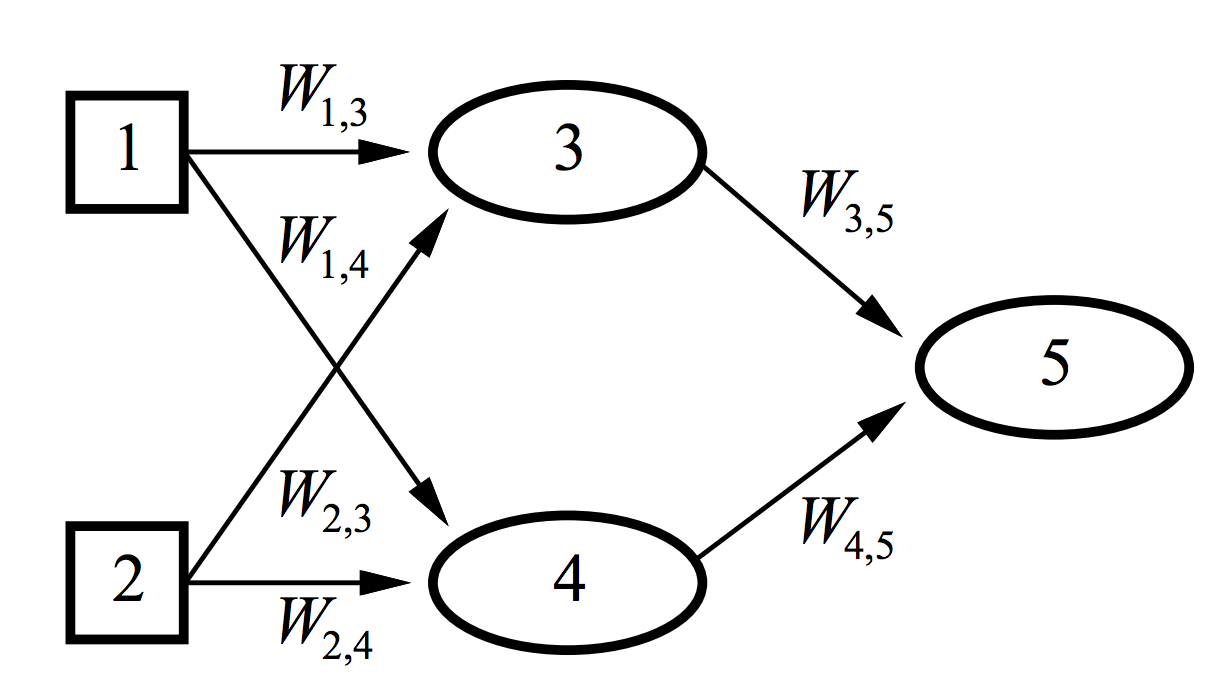
\includegraphics[width=.7\textwidth]{red_neuronal}
\end{figure}

La idea de las redes neuronales es que sean capaces de aprender funciones
generalizando ejemplos de entradas y salidas de la función. Un algoritmo de
aprendizaje para redes neuronales deberá ajustar los pesos de la red de tal
manera que se minimice alguna medida del error producido sobre el conjunto de
entrenamiento \parencite{russel_norvig}.


\subsection{Propagación hacia atrás}
\label{sec:backprop}

El algoritmo usado para entrenar la red se llama propagación hacia atrás. Se
trata de actualizar los pesos de la red para reducir el error, entendido como
la diferencia entre la salida de la red con la salida esperada.

Para actualizar los pesos se usa el descenso del gradiente. Cada peso que lleva
a una neurona de salida se actualiza de la siguiente manera: 
\[
    W_j \leftarrow W_j + \alpha \times Err \times g'(in) \times x_j
\]

Siendo $W_j$ el peso, $\alpha$ la tasa de aprendizaje, $Err$ el error cometido
en la salida, $g'$ la derivada parcial de la función de activación y $x_j$ la
entrada. Si el error es positivo, la salida de la red es demasiado pequeña y por
ello los pesos se incrementan para las entradas positivas y se decrementan para
las entradas negativas. Cuando el error el negativo ocurre lo contrario.

Para actualizar los pesos de las neuronas ocultas se define una función de
actualización de pesos. Es la misma con la que se actualizan los pesos de la
capa final pero ahora se entiende que cada nodo oculto es responsable de una
fracción del error en cada nodo de salida, proporcional al peso que tenga la
conexión entre ambos nodos. Así que los valores se propagan hacia atrás con la
fuerza de la conexión entre el nodo de salida y el nodo oculto.

\subsection{Codificación \textit{onehot}}

La codificación \textit{onehot} es la representación de variables categóricas
como un vector binario. Cada elemento del vector representa la pertenencia a
una de las categorías disponibles en el problema. El vector final tendrá el
mismo tamaño que la cantidad de categorías y estará completo de ceros, excepto
en el lugar perteneciente a la categoría del elemento, donde contendrá un uno.

Esta codificación es útil para redes neuronales, ya que al trabajar con varias
categorías es más eficiente tener una neurona de salida para cada categoría
disponible, en vez de trabajar con combinaciones de menos neuronas.


\section{Imágenes digitales}

Una imagen en el ámbito digital se entiende como una matriz de puntos.
Cada uno de estos puntos puede ser interpretado como un número real entre 0 y 1, que representa la localización de este punto en la escala de grises. En esta representación usaremos valores menores para los puntos más oscuros y valores mayores para puntos más claros.

Un ejemplo de esa representación es la matriz de la figura \ref{Seven_number}, que representa la imagen de la figura \ref{Seven_corner}.

\begin{figure}
    \centering
    \caption{\textit{Imagen parcial en blanco y negro de un dígito escrito a mano}}
  \label{Seven_corner}
  
\includegraphics[width=.6\textwidth]{Seven_corner}
\end{figure}

\begin{figure}
    \centering
    \caption{\textit{Matriz que representa los valores de cada punto en la imágen de la figura \ref{Seven_corner}}}
  \label{Seven_number}
  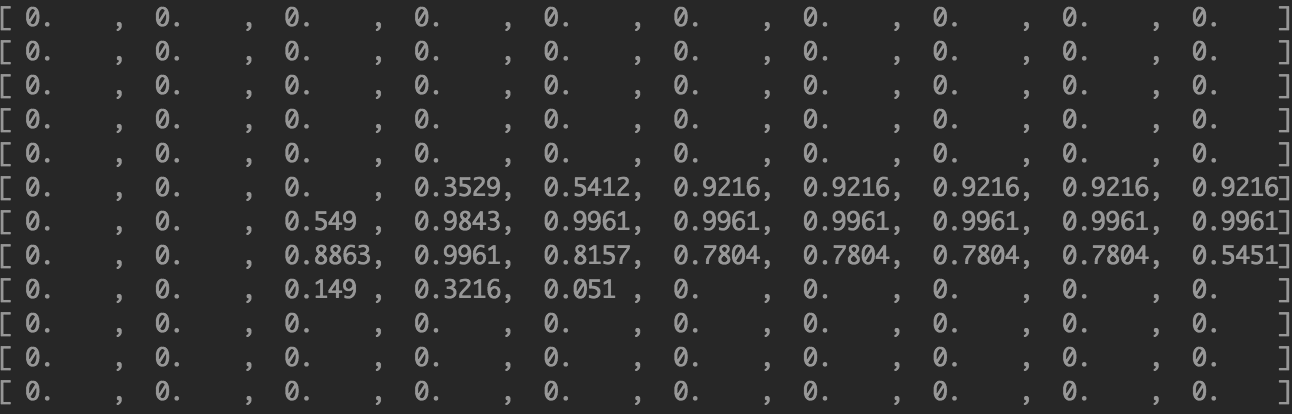
\includegraphics[width=\textwidth]{Seven_number}
\end{figure}


En imágenes en color se suele usar el sistema \textit{RGB (Red, Green, Blue)} para representar diferentes colores en cada punto de la imagen. En vez de usar un solo valor por punto se usan tres valores, cada uno representando la intensidad del color rojo, verde y azul en ese punto. Superponiendo estos tres valores se consigue el color final. Por lo tanto, las imágenes \textit{RGB} constan de tres matrices, cada una con los valores reales entre 0 y 1 para cada color.

Para simplificar, algunos ejemplos de esta memoria van a usar una escala de grises, pero son aplicables a imágenes en color aplicando las operaciones a las tres diferentes matrices al mismo tiempo.

\section{Filtros convolucionales}

Al trabajar con esta interpretación de lo que es una imagen, se pueden usar operaciones sobre la matriz de la imagen para transformarla de diferentes maneras.

Consideremos por ejemplo la siguiente matriz 3$\times$3 (llamada matriz filtro de convolución):

\[
  F=
  \left[ {\begin{array}{ccc}
   -1 & -1 & -1 \\
   1 & 1 & 1 \\
   0 & 0 & 0 \\
  \end{array} } \right]
\]

Se puede usar $F$ como un filtro para una imagen de la siguiente manera: primero, superponemos la matriz en algún punto de la imagen. Esto modificará el pixel donde ha quedado colocado el valor central de la matriz F. Para ello multiplicamos cada uno de los valores superpuestos, sumamos los resultados y los sustituimos en el valor central. Esto se hace para cada píxel de la imagen original (superponer el filtro en ese píxel y sustituir el valor por la operación).

En los bordes de la matriz existen menos píxeles adyacentes a cada píxel: seis en los bordes y tres en las esquinas. Para que la operación se haga con la misma cantidad de elementos se presupone que todos los valores que no existen son 0.

En el caso de la matriz F, la fila superior son todos valores negativos, la intermedia son todos 1 y la inferior todos ceros. Si aplicamos entonces la operación descrita sobre una imagen, los píxeles más brillantes (aquellos con mayor valor) en la imagen resultante serán los que su fila superior es cero, eliminando los valores negativos y su fila intermedia es 1. 

Esto ocurrirá con más frecuencia en los bordes superiores de objetos claros con fondo oscuro.

Para mostar la utilidad de los filtros, los aplicaremos a la imagen de un dígito escrito a mano, sacado de la base de datos MNIST \parencite{lecun-mnisthandwrittendigit-2010}, que incluye 70000 imágenes de dígitos alfanuméricos escritos a mano.

\begin{figure}
    \centering
    \caption{Imágen de un dígito escrito a mano, sacado de la base de datos MNIST}
  \label{seven}
  
\includegraphics{seven}
\end{figure}

Si aplicamos el filtro F a la imagen de la figura \ref{seven} podemos observar cómo resalta en blanco los bordes superiores y en negro los inferiores. Véase la primera columna de la figura \ref{filters}. Filtros similares, rotando los valores del filtro F, son capaces de resaltar bordes laterales u oblicuos (resto de columnas de la figura \ref{filters}).

\begin{figure}
    \centering
    \caption{Aplicación de diferentes filtros a la imagen de la figura \ref{seven}}
  \label{filters}
  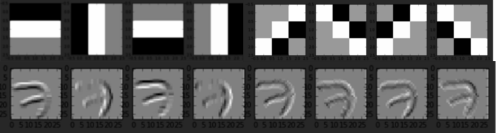
\includegraphics{filters}
\end{figure}

Lo interesante de este método es que hemos conseguido resaltar características
del objeto representado en la imagen usando solo operaciones matriciales.

Las matrices de convolución pueden ser de mayor tamaño, permitiendo capturar
características más complejas. La matriz 3$\times$3 es la menor matriz que
permite definir en su totalidad el concepto de espacio, pudiendo extraer
características espaciales en dos dimensiones.

A la hora de trabajar con imágenes en color es necesario aplicar cada filtro a
cada capa del modelo RGB por separado, permitiendo de esta manera detectar diferentes
características de la imagen que ocurran solo en uno de los colores.

Para analizar cómo afectan diferentes filtros a una imagen, en la página \parencite{visualizer_convolution} se pueden probar ejemplos con filtros personalizados, haciendo el concepto mucho más sencillo de comprender.

\section{Redes neuronales convolucionales}
\label{sec:conv-net}

Hemos explorado la idea de que determinados filtros sean capaces de extraer información localizada sobre características de la imagen. En el ejemplo del apartado anterior, dada una imagen podíamos saber si había bordes superiores y dónde se podían encontrar. Esto puede ser de gran utilidad en el campo del reconocimiento de imágenes, ya que podemos usar esa información localizada para categorizar o aplicar otro tipo de técnicas en esas áreas señaladas. El problema radica en encontrar los mejores filtros para que extraigan las características más relevantes de una imagen.

Analizando cómo funcionan los filtros convolucionales vemos su parecido con las redes neuronales. Al igual que estas, los filtros se pueden entender como funciones que al aplicarse a los datos de entrada producen unos datos de salida que serán más o menos relevantes para el objetivo buscado. El entrenamiento de una red neuronal va modificando los pesos de las diferentes capas hasta que produce una salida relevante para cada ejemplo del conjunto de entrenamiento. Si entendemos los pesos como matrices convolucionales, podemos hacer que sea la propia red la que busque el mejor filtro para nuestro problema de clasificación. De hecho, ya que las redes neuronales son capaces de componer diferentes funciones en diferentes capas de la red para aprender funciones no lineales, podemos aplicar la misma idea a las redes con filtros: componer diferentes filtros para poder extraer características más complejas.

En esta idea se basan las redes convolucionales que trabajan con imágenes. Cada capa de la red constará de varios filtros que se aplicarán a las imágenes que reciba, proporcionando los resultados a la siguiente capa. Ya que lo que importa es la composición de filtros, cada capa deberá entrenar varios filtros al mismo tiempo, permitiendo así aumentar la combinatoria final.

De esta manera, los pesos de cada capa vendrían dados en una matriz tridimensional, que se puede entender como $d$ (profundidad) filtros de dimensión  $w \times h$ (anchura y altura), como se indica en la figura \ref{cnn_basic}.

\begin{figure}
    \centering
    \caption{\textit{Ejemplo de dos representaciones de la misma red convolucional. Abajo el modelo resumido con cajas.}}
  \label{cnn_basic}
  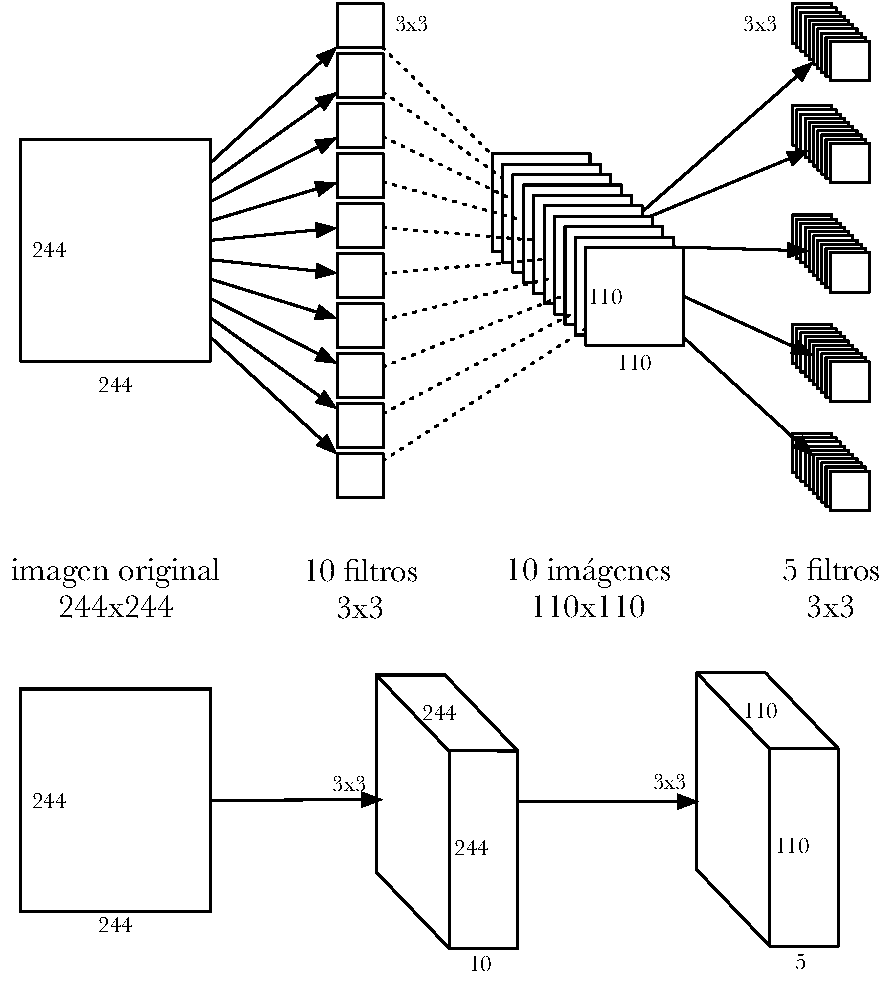
\includegraphics[width=.7\textwidth]{cnn}
\end{figure}


\subsection{Estructura de una capa convolucional}

El concepto de capa en una red convolucional incluye una agrupación de diferentes capas que efectúan diferentes operaciones. Como en las redes neuronales clásicas, la capa precisará de un tratamiento de las entradas con los pesos (en este caso los filtros convolucionales) y una función de activación.

\subsubsection{Capa convolucional - CONV \textit{(Convolutional layer)}}

Las capas convolucionales son las que hemos visto hasta ahora. Tendrán como pesos $n$ filtros convolucionales (todos del mismo tamaño) y producirán las $n$ imágenes resultantes de aplicar estos filtros a la imagen de entrada. Por ejemplo, de una imagen de tamaño $32\times 32$ proporcionada a una capa convolucional de 8 filtros se obtendrá una salida de tamaño $32 \times 32 \times 8$, o lo que es lo mismo, 8 imágenes $32 \times 32$.

\subsubsection{Capa de activación - RELU \textit{(Rectifier Linear layer)}}
\label{sec:relu}

Al igual que en las redes clásicas es necesario tratar la salida de la
aplicación de los pesos sobre las entradas con una función de activación. En el
caso de las redes convolucionales la función de activación se aplica a cada
píxel resultante del filtro.

La manera habitual de modelizar la salida de una neurona en las RNAs es a
través de $f(x) = tanh(x)$ o $f(x) = (1 + e^{-x})^{-1}$ (función sigmoide). A
la hora de entrenar la red con descenso del gradiente, estas funciones son
mucho más lentas que otra función que también evita la linealidad: $f(x) =
max(0, x)$, llamada ReLU (\textit{Rectifier Linear}). Las redes neuronales
convolucionales entrenan varias veces más rápido usando ReLU  que las
equivalentes usando la función $tanh$ (ver figura \ref{relu-vs-tanh}).

\begin{figure}
    \centering
    \caption{Evolución de un entrenamiento para una red convolucional de cuatro capas usando ReLUs (línea sólida) vs usando tanh (línea discontínua) \parencite{krizhevsky2012imagenet}}
  \label{relu-vs-tanh}
  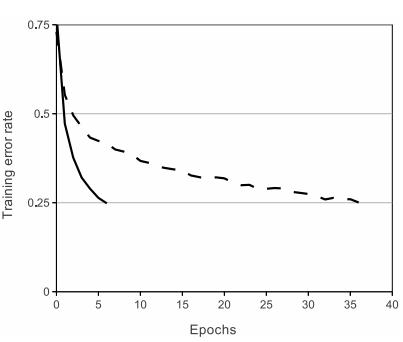
\includegraphics[width=.6\textwidth]{relu-vs-tanh}
\end{figure}

\subsubsection{Capa de muestreo - POOL \textit{(Pooling layer)}}

Al usar convoluciones en una imagen, la información del entorno de cada punto
queda difuminada y redundante. Gracias a esto se puede reducir el tamaño del
problema mediante muestreo. Las capas de muestreo (\textit{pooling layers})
resumen las salidas del entorno de cada grupo de neuronas. Un ejemplo de
función de muestreo sería elegir el valor máximo de cada cuadrado de 4 píxeles
(figura \ref{maxpool}).

Si la salida de una capa CONV + RELU es $32 \times 32 \times 8$, al aplicar la capa de muestreo la salida se convertirá en $16 \times 16 \times 8$. Al eliminar el 75\% de las activaciones se reducen la cantidad de parámetros y el tiempo de computación, y además ayuda a reducir el sobreajuste.

\begin{figure}
    \centering
    \caption{\textit{Max-pooling sobre una imagen de $4\times4$}}
  \label{maxpool}
  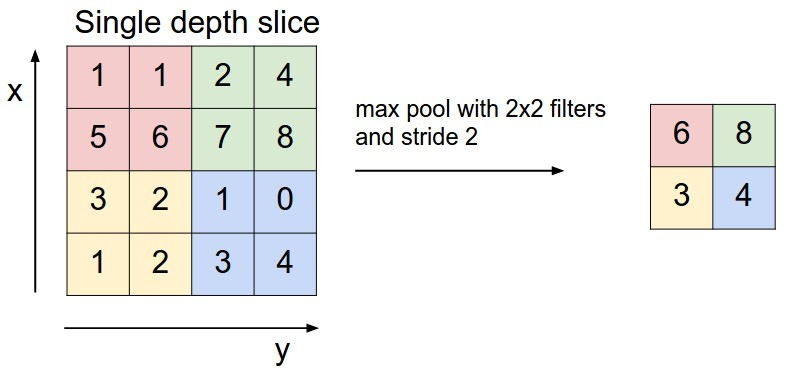
\includegraphics[width=.6\textwidth]{maxpool}
\end{figure}

\subsubsection{Capa densa - FC \textit{(Fully connected layer)}}

Esta capa es una capa clásica de red neuronal. Su función es calcular las probabilidades de clasificación dadas las imágenes tratadas. Cada neurona de esta capa estará conectada a cada una de las activaciones de la capa anterior, produciendo una salida por cada clase a clasificar.

Esta capa suele usarse al final de la arquitectura, cuando se han producido varios ciclos de capas convolucionales (CONV + RELU + POOL). Sin embargo, también es común ver arquitecturas con varias capas FC conectadas al final, ampliando la flexibilidad de clasificación de la red en base a características extraidas.

\subsection{Arquitectura}
\label{sec:conv-net-arch}

\begin{figure}
    \centering
    \caption{Ejemplo de arquitectura de una red convolucional para clasificación, \parencite{clarifai}}
\label{conv-arch}
  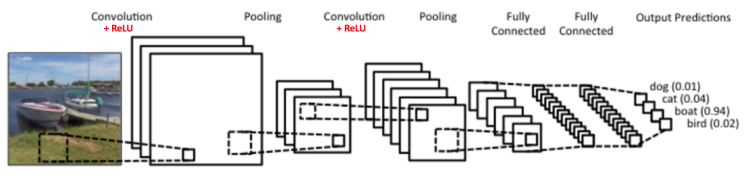
\includegraphics{conv-arch}
\end{figure}

Un esquema simplificado de un ejemplo de uso de las capas mencionadas se puede encontrar en la figura \ref{conv-arch}. La idea es, mediante capas CONV + RELU + POOL, transformar la imagen en una multitud de representaciones de conceptos cada vez más abstractos. Una vez se alcancen dichos conceptos, usar capas FC para modelizar la salida de la red.

Como se verá en la solución presentada para este proyecto, en el capítulo \ref{cap:soluciones}, usar esta arquitectura permite apoyarse en determinadas estrategias para mejorar la eficacia del modelo predictivo.
 
% Chapter Template

\chapter{Definición del problema}

\label{Chapter5} % Change X to a consecutive number; for referencing this chapter elsewhere, use \ref{ChapterX}

%----------------------------------------------------------------------------------------
%	SECTION 1
%----------------------------------------------------------------------------------------

\section{Kaggle}

Kaggle es una plataforma donde se organizan competiciones de modelos predictivos o de aprendizaje automático sobre un problema real. Diferentes organizaciones plantean un problema y ofrecen un premio para el mejor modelo que lo resuelva, haciendo que miles de participantes prueben ideas diferentes y consigan puntos de vista que, en organizaciones tradicionales, un solo equipo no tendría.

En este trabajo se ha optado por la participación en uno de esos problemas, The Nature Conservancy Fisheries Monitoring.

\section{The Nature Conservancy Fisheries Monitoring}

En el océano pacífico, donde se captura más del 60\% del atún del mundo, tienen lugar prácticas de pesca irregular que amenazan a los ecosistemas marinos y a la estabilidad de la pesca mundial. The Nature Conservancy es una asociación que trabaja con organizaciones locales y globales para preservar las especies marinas de cara al futuro.

La principal idea para controlar la pesca y explotación de recursos marinos es el uso de cámaras en barcos, que ayudan a monitorizar las actividades pesqueras de estos. Aunque funciona muy bien como sistema de control, la cantidad de datos e imágenes generadas hace que sea muy costoso de procesar manualmente.

\begin{center}
  \makebox[\textwidth]{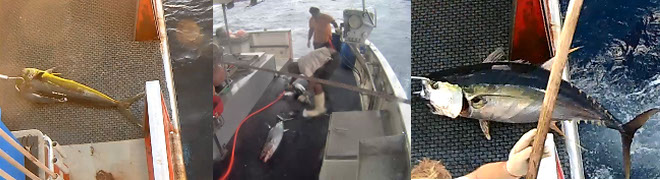
\includegraphics[width=\linewidth]{kaggle-competition-banner}}
\end{center}

La idea de este reto es desarrollar algoritmos que detecten y clasifiquen automáticamente especies de atunes, tiburones y otras especies que estos barcos pesqueros cazan. El hecho de que se pueda analizar este tipo de imágenes de una manera rápida y automática permitirá asignar recursos de una manera mucho más efectiva para el control de este tipo de actividades. (Cita: fisheries monitoring)

\section{Definición del problema}

El problema consiste en clasificar cada una de las imágenes de un conjunto de imágenes de barcos en una de las ocho categorías disponibles. Las imágenes suelen mostrar la cubierta de un barco donde puede aparecer un pez. En base al pez que aparezca hay que clasificarlo en una de las siguientes seis categorías:

\begin{center}
  \makebox[\textwidth]{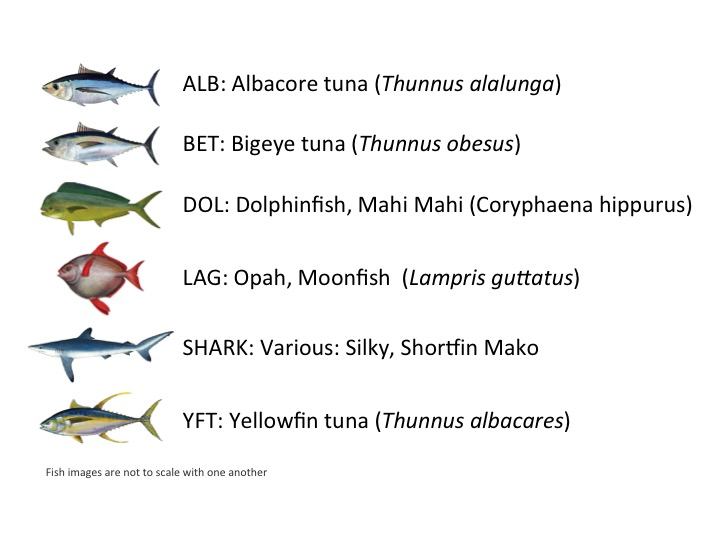
\includegraphics[width=\linewidth]{species-ref-key}}
\end{center}

En caso de que no aparezca ningún pez en la imagen, esta tendrá la categoría NOF (No Fish). Y si aparece un pez en la imagen pero no perteneciente a ninguna de las categorías mencionadas, la categoría será OTHER.

\[
  categories =
  \left[ALB, BET, DOL, LAG, SHARK, YFT, OTHER, NOF]
\]

\subsection{Datos}

El descargable que se provee en el reto consta de tres elementos:

\begin{enumerate}
  \item{Conjunto de datos de entrenamiento: 3777 imágenes etiquetadas con una de las ocho categorías existentes.}
  \item{Conjunto de test y evaluación: 1000 imágenes sin etiquetar.}
  \item{Archivo de envío de prueba: Archivo CSV que muestra la estructura que debe tener el archivo con las soluciones}
\end{enumerate}

\subsection{Envío de la solución y evaluación}
\label{sec:envio-y-eval}

Para el envío de la solución hace falta clasificar las 1000 imágenes del conjunto de evaluación, indicando la probabilidad de que caiga en cada una de las ocho categorías diferentes. En la tabla \ref{submission-sample} se muestra un ejemplo de las primeras filas del archivo CSV a enviar.

\begin{table}[]
\centering
\caption{Ejemplo del archivo de envío}
\label{submission-sample}
\begin{tabular}{lllllllll}
image          & ALB   & BET   & DOL   & LAG    & NoF   & OTHER & SHARK  & YFT  \\
img\_00005.jpg & 0.455 & 0.052 & 0.030 & 0.0173 & 0.123 & 0.079 & 0.046 & 0.194\\
img\_00007.jpg & 0.455 & 0.052 & 0.030 & 0.0173 & 0.123 & 0.079 & 0.046 & 0.194\\
img\_00009.jpg & 0.455 & 0.052 & 0.030 & 0.0173 & 0.123 & 0.079 & 0.046 & 0.194
\end{tabular}
\end{table}

El envío se evalúa usando multi-class logarithmic loss. Cada imagen ha sido etiquetada con una clase, pero es necesario enviar las probabilidades de cada clase para cada imagen. La formula final es:

\[
  logloss =
  - \frac{1}{N} \sum_{i=1}^N \sum_{j=1}^M y_{ij} \log \, p_{ij}
\],
 siendo N el número de imágenes en el conjunto de test, M el número de clases, $y_{ij}$ es 1 si la observación $i$ pertenece a la clase $j$ y 0 si no pertenece y $p_{ij}$ la probabilidad predecida de que el elemento $i$ pertenezca a la clase $j$.

 \subsecion{Leaderboard y fases de la competición}

 Existe una tabla donde se publican los resultados de los envíos de cada participante. Estos resultados están calculados solo con un subconjunto del conjunto de test, de esta manera se evita que los participantes puedan aprovechar un sobreajuste para subir en la clasificación.

La puntuación final vendrá determinada por la puntuación de todo el conjunto de test.

Esta manera de evaluar es algo bastante común en kaggle, sin embargo los organizadores de este reto en particular han decidido hacer un pequeño cambio a la hora de evaluar la puntuación.

\subsection{Doble fase de evaluación y envío}

La evaluación en este reto contará de dos partes. La primera, donde se entrenará el modelo, requiere (como ya se ha dicho) evaluar el conjunto de test de mil imágenes. La fecha límite para la entrega de modelos de esta primera fase es siete días antes de la finalización del reto. Será necesario enviar el CSV con las predicciones y el modelo usado.

Una vez finalice la primera fase, un segundo conjunto de test de muchas más imágenes será hecho público. Este conjunto de test deberá ser evaluado con el modelo generado en la fase anterior, siendo razón de descalficación modificar el modelo. Todos los participantes que no envíen la predicción de la segunda fase serán eliminados del reto.

\section{El conjunto de datos}

Aqui hago un pequeño análisis del conjunto de datos, la distribución de imágenes por clases, por estructura (tamaño de imaggen), color, etc

 
% Chapter Template

\chapter{Soluciones presentadas} % Main chapter title
\label{cap:soluciones} % Change X to a consecutive number; for referencing this chapter elsewhere, use \ref{ChapterX}

\section{Metodología}
\label{sec:metodology}

La puntuación final de la competición será calculada mediante una función de
pérdida logarítmica, como vimos en el apartado \ref{sec:envio-y-eval}. Al no
tener las categorías del conjunto de datos de test debemos delegar el cálculo de
la puntuación en \textit{Kaggle}, que permite enviar hasta cinco predicciones al
día. Esto es un obstáculo para hacer pequeñas pruebas e iterar rápido sobre los
resultados. Por otra parte, el conjunto de test de la segunda fase tiene más de
13000 imágenes, que no son rápidas de cargar en memoria ni de pasar por el
modelo. En determinados casos la evaluación del segundo conjunto de test ha
tardado más de 6 horas.

La solución a este problema se ha resuelto usando un subconjunto del conjunto
de entrenamiento dedicado solo a la evaluación de modelos. Por otra parte, para
el entrenamiento es necesario usar un subconjunto de validación, por lo tanto
es necesario dividir el conjunto de entrenamiento original en tres
subconjuntos: entrenamiento, validación y test. La partición se ha realizado
dejando un \textbf{60 \%} de los datos al conjunto de entrenamiento, un
\textbf{20 \%} al conjunto de validación y un \textbf{20 \%} al conjunto de
test.

Otra posibilidad sería emplear la metodología de validación cruzada, que
consiste en dividir el conjunto de entrenamiento en $n$ partes, usando $n-1$ de
ellas para el entrenamiento y la restante para la validación. Esto se repite
$n$ veces, considerando en cada una de ellas uno de los subconjuntos como
conjunto de validación. La bondad del modelo será el valor medio de todos los
modelos generados. No obstante, en los algoritmos de redes convolucionales con
imágenes no se suele usar la validación cruzada, ya que son algoritmos muy
costosos y puede aumentar mucho el tiempo de entrenamiento.

\subsection{Partición del conjuntos de datos} 

La partición de un conjunto de datos es una operación delicada. Ya vimos que
uno de los problemas de nuestro conjunto de datos de entrenamiento era que la
cantidad de imágenes para cada clase era muy variada, teniendo algunas de ellas
un número muy bajo de ejemplos. Si seleccionamos aleatoriamente el 40 \% de las
imágenes, es posible que no se elijan ejemplos de una o varias de las
categorías, con lo que los modelos construidos no las tendrían en cuenta.

La solución adoptada ha sido realizar un muestreo estratificado para realizar la partición del conjunto de datos. Este consiste en realizar la partición de cada clase por separado, siguiendo la proporción 60 \% - 20 \% - 20 \% indicada anteriormente.

\subsection{Evaluación del modelo}

Para una búsqueda más eficiente de parámetros y configuraciones los modelos se evaluarán previamente usando nuestro subconjunto de test local. Aquellos modelos que resulten especialmente interesantes por tener una puntuación máxima local entre aquellos a los que se compara se subirán entonces a \textit{Kaggle} para su evaluación usando el conjunto de test correspondiente a la fase en la que nos encontremos.

\textit{Kaggle} usa la pérdida logarítmica para medir la bondad de cada modelo (sección 
\ref{sec:envio-y-eval}). Esta métrica se verá perjudicada si puntuamos con una probabilidad muy baja la categoría correcta de la imagen. Una técnica para tratar de aliviar este problema consiste en truncar las probabilidades de cada clase, tanto en su valor máximo como en el mínimo. En nuestro caso vamos a hacer que las probabilidades superiores a 0.95 se trunquen a 0.95 y las inferiores a 0.15 se trunquen a 0.15.


\subsection{Software}

Todos los modelos de redes convolucionales construidas en este proyecto han sido entrenados usando \textit{Keras} (véase apéndice \ref{ap:keras}) sobre cuadernos de \textit{Jupyter} \parencite{jupyter}. La estructura de desarrollo y algunas utilidades están descritas en \parencite{fastai} y \parencite{felixyu}.


\section{Arquitectura de los modelos}

Los humanos somos expertos en la identificación visual. Esto se debe, en
parte, a que nos llevamos la mayor parte de nuestra vida resolviendo problemas
de identificación visual y somos muy eficientes generalizando las
características de una imagen.

La competición de reconocimiento visual a gran escala de \textit{ImageNet},
conocida por sus siglas ILSVRC (\textit{Imagenet Large Scale Visual Recognition
Challenge}) \parencite{ILSVRC} es una competición de reconocimiento de imágenes
que pretende seguir el progreso alcanzado por los modelos de inteligencia
artificial a la hora de identificar y generalizar elementos de una imagen. En
esta competición se deben detectar elementos en 150000 fotografías y
clasificarlos en una entre 1000 categorías diferentes.

En 2010 y 2011 los modelos ganadores consiguieron una tasa de error de un 28,2 \% y un 25.8 \%, respectivamente. En 2012, el modelo presentado en \parencite{krizhevsky2012imagenet}, una red convolucional profunda, ganó con una tasa de error del 16.4 \%, superando en casi un 10 \% al segundo clasificado. Esta victoria hizo que el enfoque de esta propuesta haya sido usado por los ganadores de los años siguientes.

En este trabajo se pretende aprovechar la capacidad de generalización de los modelos ganadores del ILSVRC. Es decir, no se construirá una red convolucional con una estructura similar a la de \parencite{krizhevsky2012imagenet}, sino que se utilizará esa misma red adaptándola a nuestro problema.

\subsection{Red convolucional}

La figura \ref{general-architecture} representa la red usada en ILSVRC 2012, la
cual se compone de una red convolucional para la extracción de características
de la imagen, seguida de una red densa para la clasificación de la imagen
usando esas características extraídas.

\begin{figure}
  \caption{Arquitectura de una red convolucional profunda. Consta de una acumulación de capas convolucionales destinadas a extraer características de la entrada y una serie de capas densas para clasificar la entrada usando dichas características.}
\label{general-architecture}
  \makebox[\textwidth]{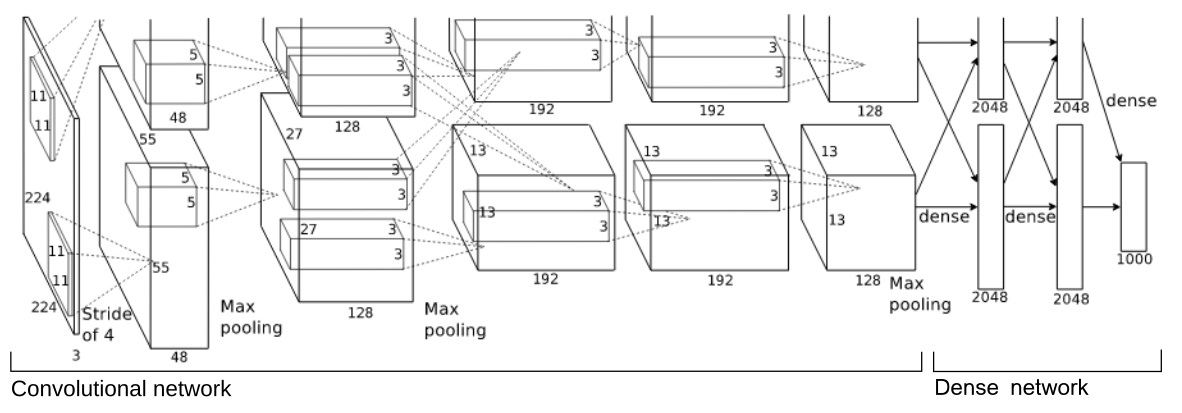
\includegraphics[width=\linewidth]{imagenet-arch}}
\end{figure}

Como explicamos en la sección \ref{sec:conv-net}, cuando una red convolucional
recibe una imagen devuelve $N$ matrices bidimensionales representando el
resultado de la aplicación de los $N$ conjuntos de filtros a la imagen inicial.
Intuitivamente podemos pensar que la salida de cada uno de estos filtros
representa la aparición en la imagen de la característica que esté detectando
el filtro. Necesitamos entonces que en las últimas capas la red aprenda
filtros que se activen sólo con la aparición de una clase de pez.

Un detalle que debemos tener en cuenta que este modelo convolucional no ha sido entrenado con el conjunto de entrenamiento del problema, sino con el conjunto de entrenamiento de \cite{imagenet}. Por lo tanto, nuestro uso de esta red convolucional será únicamente para transformar cada imagen del conjunto de entrenamiento del problema a un conjunto de características.

La arquitectura del artículo original \parencite{krizhevsky2012imagenet} usa
capas convolucionales donde alterna filtros de $11\times11$, $5\times5$ y
$3\times3$, el cual parece una buena elección para usar como modelo
convolucional preentrenado. Sin embargo, la aplicación de este trabajo es una
competición internacional donde se usarán soluciones \textit{state of the art}.
El modelo de la figura \ref{general-architecture} representa el ganador de la
edición 2012 de la competición ILSVRC, hace ya cinco años, por lo que resulta
conveniente analizar cuales fueron los ganadores de años posteriores.

El modelo principal que usaremos es VGG, desarrollado por el \textit{Visual
Geometry Group}, de la Universidad de Oxford \parencite{simonyan}. Es un modelo
especialmente interesante por su simplicidad, aparte de obtener una de las
mejores puntuaciones en ILSVRC 2014. Una de las principales características de
VGG es la idea de que los filtros convolucionales mayores de $3\times3$, como
por ejemplo los de $5\times5$ u $11\times11$, pueden ser representados por
combinaciones de filtros $3\times3$.

De las configuraciones descritas en \parencite{simonyan} hay una que sobresale
por su eficiencia, llamada VGG16. Usando un total de trece capas CONV con
filtros de $3\times3$, cinco capas POOL y tres capas FC (de 4096, 4096 y 1000
salidas), seguida de una función \textit{softmax} (figura \ref{vgg16-arch}), es
capaz de mejorar la eficacia del modelo de Krizhevsky. El nombre de esta
configuración es VGG16, por ser esta la cantidad de capas CONV y FC que posee.

\begin{figure}
  \caption{Arquitectura de VGG}
\label{vgg16-arch}
  \makebox[\textwidth]{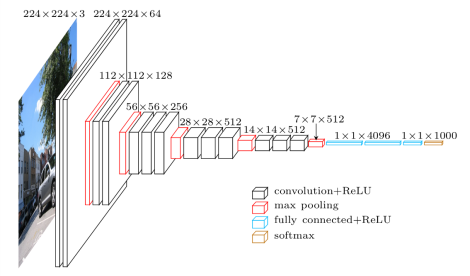
\includegraphics[width=.7\linewidth]{vgg16-arch}}
\end{figure}

\subsection{Ajuste fino}

Si observamos la última capa del modelo VGG16, vemos que la salida tiene 1000
elementos. Tiene esta forma ya que ILSVRC consiste en clasificar una imagen
entre mil categorías diferentes. Como en nuestro problema solo tenemos ocho
categorías, es lógico modificar esta última capa para que únicamente tenga ocho
salidas.

Al modificar la estructura de la última capa estamos destruyendo pesos y
haciendo que muchos de los que ya existían carezcan de sentido. El hecho de que
VGG una esta separación lógica entre la red convolucional y la red densa hace
que se pueda separar el modelo en dos submodelos diferentes: uno convolucional,
que no habrá cambiado con la adaptación a las ocho categorías, y otro denso,
que tendrá que ser entrenado de nuevo.

Esta técnica de ajustar los parámetros de un modelo ya conocido para adaptarlo
a un nuevo conjunto de datos se conoce como ajuste fino (\textit{fine-tuning}).
En la figura \ref{basic_architecture} se puede ver un resumen de las diferentes
etapas por los que pasa la red.

Al dividir la red en dos subredes diferentes hay que tener en cuenta que la
segunda, la red densa, no recibe como entrada las imágenes, sino la salida de
la primera red convolucional, con todas las transformaciones que esta produce.
Es necesario entonces aplicar la red convolucional a nuestro conjunto de datos
de entrenamiento para crear un nuevo conjunto de datos con el que reentrenar la
red densa.

\begin{figure}
  \caption{Estructura del modelo final. Como recibe como entrada imágenes de 244 píxeles, pasa por las diferentes redes y devuelve el vector de ocho categorías.}
\label{basic_architecture}
  \makebox[\textwidth]{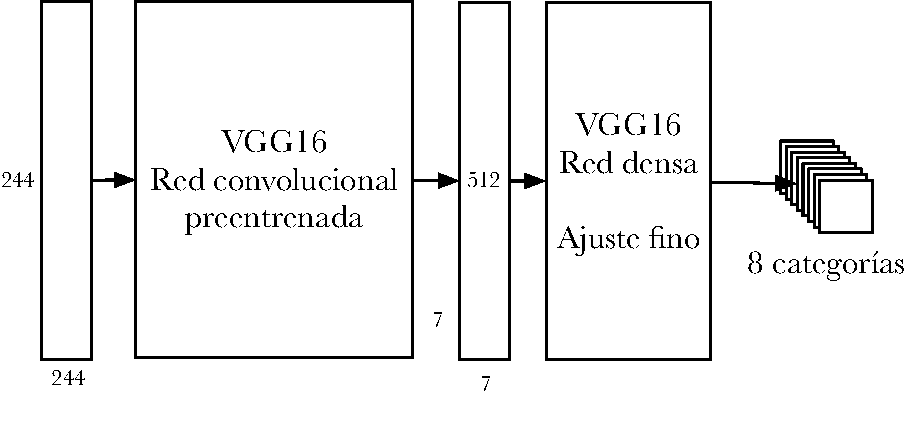
\includegraphics[width=.7\linewidth]{basic_architecture}}
\end{figure}

El siguiente código (simplificado) realiza esta tarea para los subconjuntos
locales de entrenamiento, validación y prueba.

\begin{python}
# Carga del modelo VGG16
from vgg16 import Vgg16
model = Vgg16()

# Separacion entre red convolucional y densa
import utils
conv_model, dense_model = utils.split_at(model, MaxPooling2D)

# Carga de los diferentes conjuntos de datos
#  'path' es la carpeta donde se encuentra los
#  conjuntos de datos
train, train_labels = get_data(path + 'train')
valid, valid_labels = get_data(path + 'valid')
test, test_labels = get_data(path + 'test')

# Conversion a caracteristicas mediante la red convolucional
train_feat = conv_model.predict(train)
valid_feat = conv_model.predict(valid)
test_feat = conv_model.predict(test)

# Sustitucion de la capa de salida
dense_model.pop()  # Eliminar la capa final
dense_model.add(
    Dense(8, activation='softmax')  # Introducir una nueva capa
)

# Compilacion del modelo
dense_model.compile(
    SGD(lr=0.01),  # Factor de aprendizaje
    loss='categorical_crossentropy',
    metrics=['accuracy'],  # Muestra la precision del modelo
)

# Entrenamiento de la red
dense_model.fit(
    train_feat,
    train_labels,
    batch_size=64,  # Numero de imagenes a entrenar al mismo tiempo
    nb_epoch=7,     # Numero de iteraciones del entrenamiento
    validation_data=(valid_feat, valid_labels),
)

# Evaluar el modelo sobre el conjunto de test
dense_model.evaluate(test_feat, test_labels)
# Log loss, accuracy
>>> [1.90571456890184755, 0.66099843993759748]
\end{python}

La puntuación total para el conjunto de test local sería 1.906. 

El segundo número que devuelve la función $evaluate$ es la precisión
($accuracy$) del modelo. Al ser este un modelo de clasificación, la precisión
es el porcentaje de veces que la clase con la probabilidad máxima se
corresponde con la clase etiquetada en el conjunto de datos. En este caso la
red ha clasificado correctamente el 66 \% de las imágenes, un número muy
aceptable teniendo en cuenta que solo se ha tocado la capa final de un modelo
ajeno.

Al subir la predicción del conjunto de test a \textit{kaggle} se obtiene una
puntuación de \textbf{2.632} en la clasificación pública, mediante la pérdida
logarítmica. Hay que recordar que esta puntuación se calcula usando un
subconjunto del conjunto de test, así que la puntuación de este modelo puede
cambiar en la segunda fase.

Al subir a \textit{Kaggle} las predicciones del modelo sobre el conjunto de
prueba de la primera fase de la competición se obtuvo una puntuación de pérdida
logarítimica de 2.632. Aunque el error ha aumentado sensiblemente esto es
perfectamente normal, ya que las imágenes proporcionadas al modelo son
completamente nuevas.

\section{Modelo completamente conectado}
\label{sec:model_connected}

El modelo original de VGG usa dos capas $densas$ de 4096 neuronas para
clasificar entre mil clases diferentes. Ya que nuestro problema tiene solo ocho
clases diferentes probablemente no sea necesario usar capas tan grandes, por lo
que se procede a probar la misma estructura original, pero con capas cuatro
veces más pequeñas que las originales.

La estructura, por lo tanto, quedaría de la misma manera pero usando dos capas
densas de 512 neuronas cada una y una capa densa final de 8 (figura
\ref{standard_arch}). Para no tener que estar modificando cada vez el modelo
original cada vez que haga falta es mucho más sencillo crear un modelo nuevo
con $Keras$ y añadir todas las capas necesarias.

\begin{figure}
  \caption{Arquitectura del modelo completamente conectado}
\label{standard_arch}
  \makebox[\textwidth]{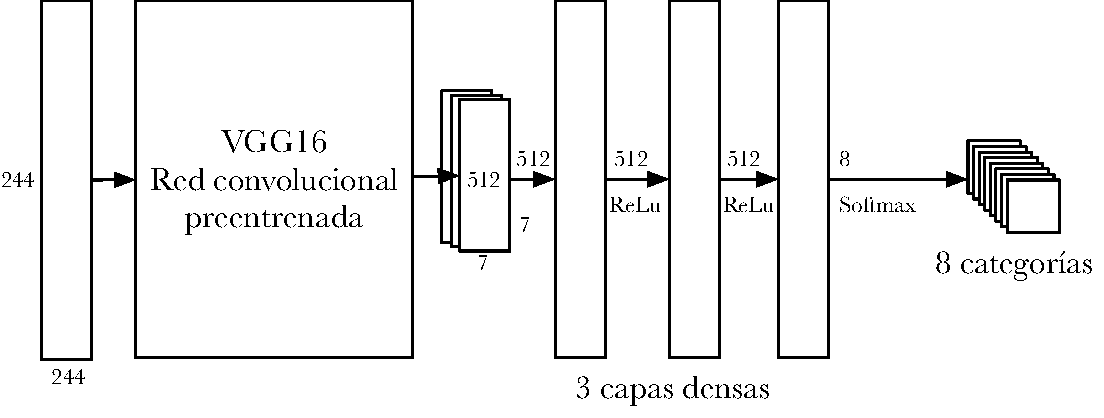
\includegraphics[width=.9\linewidth]{standard_arch}}
\end{figure}

Un paso importante a la hora de construir el modelo personalizado es tener en cuenta que las salidas de las redes convolucionales poseen tres dimensiones ($ancho \times alto \times filtros$), mientras que la redes neuronales densas poseen solo una dimensión. Es necesario convertir la salida de estas capas a una entrada permitida. \textit{Keras} ya ofrece esta posibilidad usando una capa abstracta llamada \textit{Flatten}.

\begin{python}
def list_dense_layers():
    return [
        Flatten(),
        Dense(512, activation='relu'),
        Dense(512, activation='relu'),
        Dense(8, activation='softmax')
    ]

dense_model = keras.models.Sequential(list_dense_layers())

# Entrenar la red
dense_model.compile(...)
dense_model.fit(...)

# Evaluar el modelo sobre el conjunto de test
dense_model.evaluate(test_feat, test_labels)
>>> [1.27161316430079874, 0.73067862714508579]
\end{python}

Los resultados obtenidos son ligeramente mejores que los anteriores. Sin
embargo no es aquí donde está toda la mejora. El entrenamiento de este modelo
ha sido un 80\% más rápido que el anterior (19.5 segundos por iteración en el
primero, 3.9 segundos en este último). Esto no solo ha permitido entrenar la
red durante más tiempo, sino que en el futuro hará posible entrenar sobre
mayores cantidades de datos sin aumentar excesivamente el tiempo de entrenamiento.

La puntuación en la tabla pública de \textit{Kaggle} para este modelo ha sido
de \textbf{2.381}.

\subsection{Análisis del sobreajuste}

La salida de \textit{Keras} al entrenar el modelo ofrece información de lo que
está sucediendo. Este es un ejemplo de la salida del entrenamiento del modelo
anterior.

\begin{python}
Epoch 5/7
loss: 0.354 - acc: 0.992 - val_loss: 1.091 - val_acc: 0.872
Epoch 6/7
loss: 0.253 - acc: 0.996 - val_loss: 0.995- val_acc: 0.881
Epoch 7/7
loss: 0.193 - acc: 0.997 - val_loss: 0.987- val_acc: 0.913
\end{python}

En cada una de las iteraciones del entrenamiento, \textit{Keras} muestra los
valores de aplicar el modelo actual a los ejemplos de entrenamiento y
validación. Se puede observar que el modelo funciona mucho mejor en el conjunto
de entrenamiento que en el de validación.

Cuando un modelo tiene demasiados parámetros y ha sido entrenado durante demasiado tiempo aprende a clasificar los ejemplos con los que entrena usando información específica de cada uno de ellos en vez de generalizar. Esto se conoce como \textbf{sobreajuste} (\textit{overfitting}).

Los datos del modelo anterior indican que puede existir un sobreajuste, por lo que se va a intentar tomar medidas para arreglarlo.

\subsection{\textit{Dropout}}
\label{sec:dropout}

Una de las características de VGG y otras redes convolucionales es el uso de
\textit{dropout} para reducir el sobreajuste de los modelos entrenados. El
\textit{dropout} consiste en una capa que se aplica después de las capas de
activación de las capas densas. Esta capa convierte activaciones aleatorias a
0, eliminando la información transportada (Figura \ref{dropout-net})

\begin{figure}
    \caption{A la izquierda una red neuronal estándar con dos capas ocultas. A la derecha la misma red aplicando un \textit{dropout} en cada una de las capas ocultas. Las neuronas tachadas han perdido su activación.}
\label{dropout-net}
  \makebox[\textwidth]{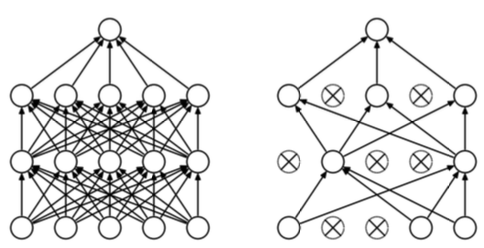
\includegraphics[width=0.7\linewidth]{dropout-net}}
\end{figure}

En un principio parecería que esto perjudica al modelo, pero al eliminar algunos de los pesos el modelo evita centrarse en características individuales de cada ejemplo de clasificación, obligándolo a generalizar más rápido \parencite{dropout}.

Un pequeño experimento en un modelo más avanzado (VGG con \textit{batch normalization} y aumento de datos) permite ver cómo afecta el \textit{dropout} a la puntuación final. En la figura \ref{dropout} se puede observar que la mejor puntuación se alcanza eliminando el 45 \% de las activaciones, consiguiendo una mejora de un 25 \% sobre el modelo que usa todas las activaciones.

\begin{figure}
    \caption{Evolución de la puntuación de un modelo usando \textit{dropout}}
\label{dropout}
  \makebox[\textwidth]{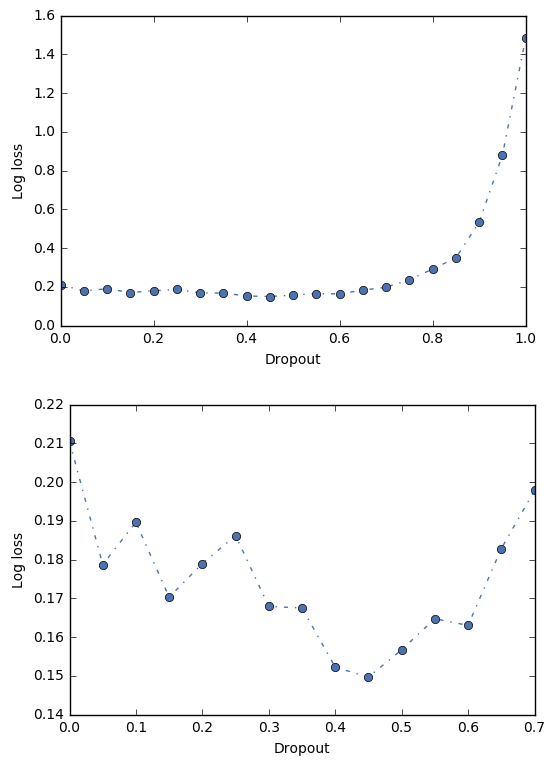
\includegraphics[width=0.7\linewidth]{dropout}}
\end{figure}

También se ve que el modelo empieza a perder eficacia a partir del 70 \% de \textit{dropout}, empeorando el modelo original. Esto significa que el modelo es capaz de generalizar con información útil incluso cuando solo posee el 30 \% de las activaciones.

Por otra parte, también es importante pensar dónde se pierden las activaciones.
Por un lado, perder demasiadas activaciones en la entrada sería el equivalente
a trabajar sin esos ejemplos. Por otro, perderlos en la salida sería aumentar
demasiado el error al clasificar, al no tener tanta capacidad de apoyo en las
otras capas.  La idea aplicada aquí es distribuir el \textit{dropout}
disminuyéndolo en la entrada y la salida y haciendo que alcance máximo
en el centro de la red.

El modelo modificado quedaría de la siguiente manera:

\begin{python}
def list_dense_layers(dropout):
    return [
        Flatten(),
        Dropout(dropout/4),  # Aplicar 1/4 del dropout definido 
        Dense(512, activation='relu'),
        Dropout(dropout),
        Dense(512, activation='relu'),
        Dropout(dropout/2),  # Aplicar la mitad del dropout definido
        Dense(8, activation='softmax'),
    ]
dense_model = keras.models.Sequential(list_dense_layers(0.45))
\end{python}

Los resultados obtenidos con esta configuracion no mejoran los resultados de la red anterior, pero como se ve en la figura \ref{dropout} sí que lo hará a posteriori, cuando se le apliquen otro tipo de modificaciones al modelo. Modelos como VGG ya incluyen \textit{dropout} (solo en las redes densas), por lo que al hacer fine-tuning con una red personalizada es necesario usarlo para mantener los resultados originales.

\subsection{Normalización por lotes}

En muchos campos del aprendizaje automático es habitual normalizar las entradas
de los modelos. Si existe una entrada mucho mayor o menor que el resto esta
puede hacer que el entrenamiento arrastre un error mayor del necesario,
produciendo inestabilidad y dificultando la convergencia del modelo. Normalizar
un conjunto de entradas hace que todas estén en la misma escala. 

El caso de las redes neuronales no es una excepción. Una entrada con un valor
demasiado grande puede llevar a tener un peso determinado demasiado grande para
contrarrestarla.

Una normalización estándar en aprendizaje automático es restar de cada entrada
el valor medio del conjunto de datos y luego dividirlo por la desviación
estándar del mismo. Esto aún presenta problemas para casos como el de este
proyecto donde se usan algoritmos como el gradiente del descenso estocástico
para la propagación hacia atrás (sección \ref{sec:backprop}).

Los modelos principales citados en este trabajo,
\parencite{krizhevsky2012imagenet} y \parencite{simonyan}, usan sus propias
técnicas de normalización, aparte de usar activaciones \textit{ReLu} (sección
\ref{sec:relu}) que son menos sensibles a los datos de entrada sin normalizar.
Sin embargo, en 2015 se presenta una técnica muy interesante de normalización
que cuadra muy bien con el gradiente del descenso estocástico: la normalización
por lotes (\textit{batch normalization}) \parencite{batch_normalization}.

La diferencia con una normalización estándar es que tras normalizar las
entradas de una capa se multiplican por un parámetro aleatorio y luego se
suma otro, cambiando así la desviación estándar y la media de la entrada. Estos
dos parámetros se hacen entonces entrenables como pesos del modelo.

Los modelos actuales que usan esta normalización por lotes consiguen la misma
precisión que los modelos sin ella usando catorce veces menos pasos de
entrenamiento \parencite{batch_normalization}.

Para aplicar esta normalización por lotes al modelo que se está entrenando hay
que añadir las capas de normalización por lotes (también disponibles en
\textit{Keras}) al modelo denso:

\begin{python}
def list_dense_layers(dropout):
    return [
        BatchNormalization(axis=1),
        Flatten(),
        Dropout(dropout/4),
        Dense(512, activation='relu'),
        BatchNormalization(),
        Dropout(dropout),
        Dense(512, activation='relu'),
        BatchNormalization(),
        Dropout(dropout/2),
        Dense(8, activation='softmax'),
    ]
dense_model = keras.models.Sequential(list_dense_layers(0.45))
\end{python}

Esto no es suficiente. A diferencia del \textit{dropout}, la normalización por
lotes sí que es capaz de mejorar la red convolucional del modelo preentrenado.
Gracias a la popularidad de esta técnica y de los modelos preentrenados que se
usan en este trabajo, ya existen entrenamientos del modelo VGG original usando
normalización por lotes, ahorrando la necesidad de entrenar una red tan grande.
Una descripción de estos entrenamientos se puede encontrar en
\parencite{pretrained_with_bn}.

En el caso de este trabajo se ha adaptado la clase $Vgg16BN$, siguiendo
los principios descritos en \parencite{fastai}. Al cambiar la red convolucional
original hay que volver a transformar el conjunto de datos que se usaba para
obtener los resultados de aplicar los filtros actualizados sobre las imágenes
de entrada.

\begin{python}
# Carga del modelo VGG16 con normalizacion por lotes
from vgg16bn import Vgg16BN
import utils
model = Vgg16BN()
conv_model, _ = utils.split_at(model, MaxPooling2D)

# Carga de los diferentes conjuntos de datos
train, train_labels = get_data(path + 'train')
valid, valid_labels = get_data(path + 'valid')
test, test_labels = get_data(path + 'test')

# Conversion a caracteristicas mediante la red convolucional
train_feat = conv_model.predict(train)
valid_feat = conv_model.predict(valid)
test_feat = conv_model.predict(test)

# Entrenamiento la red
dense_model = keras.models.Sequential(list_dense_layers(0.45))
dense_model.compile(...)
dense_model.fit(...)
# Evaluacion del modelo sobre el conjunto de test
dense_model.evaluate(test_feat, test_labels)
>>> [0.45127591543710, 0.96109451984491]
\end{python}

Como se puede apreciar, los dos últimos cambios han supuesto una mejora considerable sobre el modelo anterior, clasificando correctamente el 96\% de los ejemplos del conjunto de test.

La puntuación en la tabla pública de \textit{Kaggle} para este modelo ha sido
de \textbf{1.017}.


\subsection{Aumento de datos}

Uno de los principales obstáculos de este problema es el reducido tamaño del conjunto de datos de entrenamiento. El tener pocos ejemplos sobre los que entrenar hace que al modelo le cueste generalizar sobre los ejemplos disponibles, produciéndose un sobreajuste.

Uno de los métodos que se usan para tratar de reducir el sobreajuste del modelo es el llamado aumento de datos (\textit{data augmentation}). Consiste en generar imágenes de entrenamiento adicionales a partir de las ya disponibles, rotando la imagen original, aumentándola, cambiando ligeramente el color, etc.

En el caso de nuestro problema esta técnica es especialmente interesante, ya
que las cámaras de los barcos están fijas apuntando siempre a la misma zona. En
las fotos sobre los peces capturados estos siempre suelen estar con la cabeza
apuntando en dirección contraria al agua. Ello hace que la red reconozca más
fácilmente peces dispuestos en una determinada dirección, costándole más
trabajo para el resto de direcciones. Si las redes convolucionales ayudaban a
detectar determinados patrones en cualquier punto de la imagen, el aumento de
datos hace lo propio de otras variantes como la rotación, el tamaño o el filtro
de color dado por el ambiente.

Un ejemplo de aumento de datos se muestra en la figura \ref{augmentations}, que contiene cuatro imágenes obtenidas al reescalar de distintas maneras la imagen original de la figura \ref{aug-original}.

\begin{figure}
    \caption{Imagen del conjunto de datos}
\label{aug-original}
  \makebox[\textwidth]{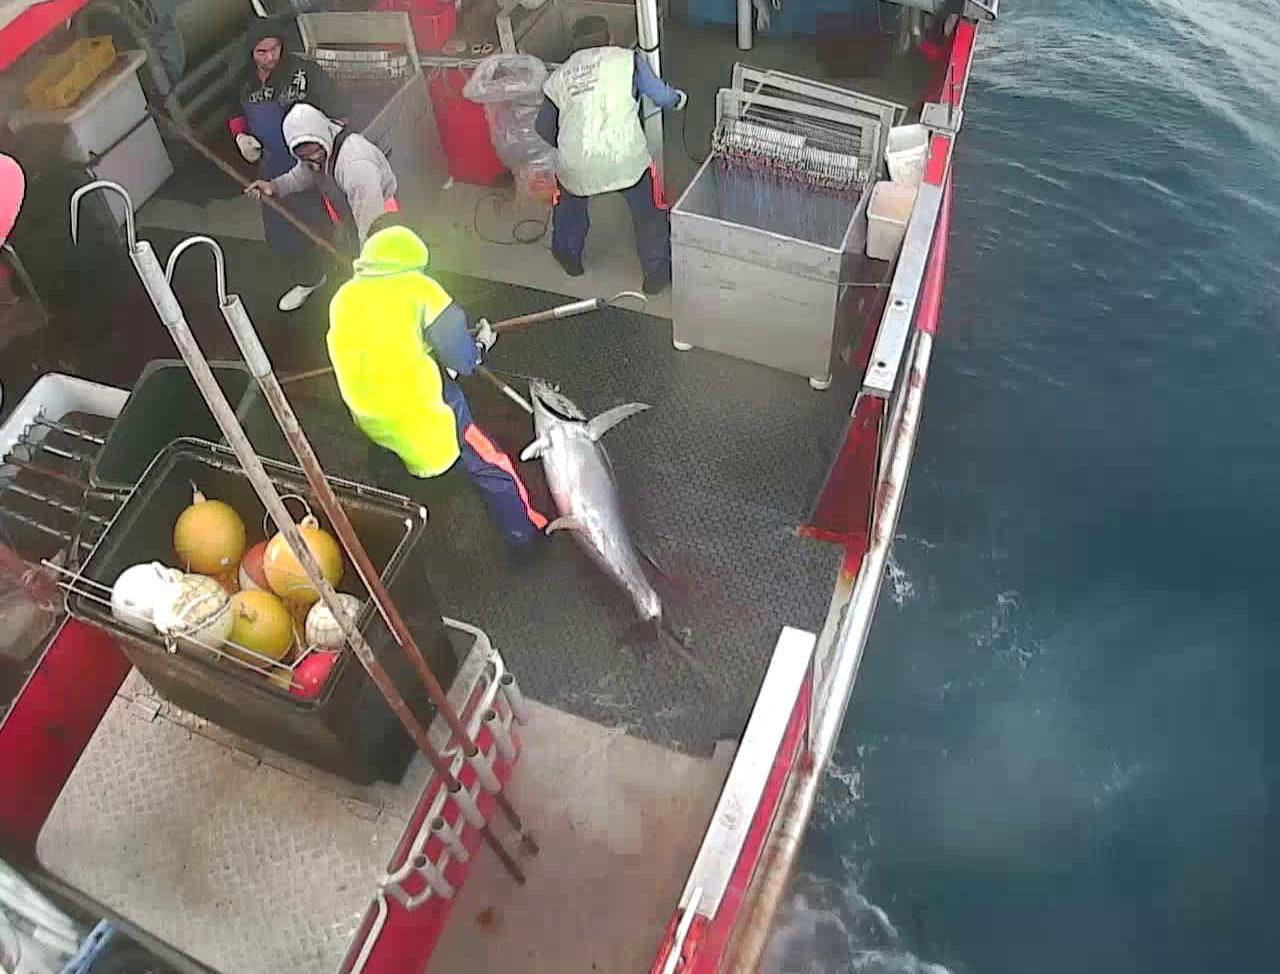
\includegraphics[width=0.7\linewidth]{aug-original}}
\end{figure}

\begin{figure}
    \caption{Cuatro aumentos diferentes de la imagen, reescalada a $224\times224$ píxeles}
\label{augmentations}
  \makebox[\textwidth]{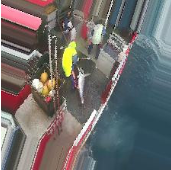
\includegraphics[width=.2\linewidth]{au1}}
  \makebox[\textwidth]{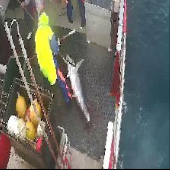
\includegraphics[width=.2\linewidth]{au3}}
  \makebox[\textwidth]{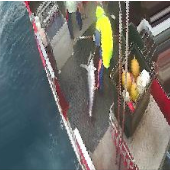
\includegraphics[width=.2\linewidth]{au2}}
  \makebox[\textwidth]{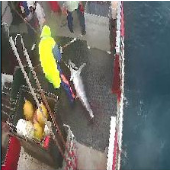
\includegraphics[width=.2\linewidth]{au4}}
\end{figure}

Para trabajar con aumentos de datos, \textit{Keras} proporciona una serie de
opciones de transformación dentro de la utilidad para importar conjuntos de
datos. Al definir dichas opciones, como por ejemplo rotación, zoom o volteo
horizontal, \textit{Keras} generará nuevas imágenes a la vez que carga el
conjunto de datos en memoria.

Si es necesario conocer cómo se aplican las transformaciones a las diferentes imágenes, es posible especificar un directorio de salida del generador de imágenes, de tal manera que los resultados de las distintas transformaciones se guarden en directorios particulares.

\begin{python}
# Creacion del generador de imagenes
image_generator = image.ImageDataGenerator(
    rotation_range=30,
    horizontal_flip=True,
    zoom_range=0.4,
)

batches = img_generator.flow_from_directory(
    path+'test_aug',
    target_size=(224,224),
    class_mode='categorical',
    shuffle=False,
    batch_size=4,
    save_to_dir=path+'augmentation',
)

# Iteracion sobre lotes para extraer los datos
# En este caso se sacan 4 veces la cantidad de datos originales
data = [batch.next() for _ in range(batches.nb_samples * 4)]
\end{python}

Ahora no es necesario modificar el modelo, solo reentrenarlo con los nuevos datos. Como ha ocurrido antes, al cambiar el conjunto de datos hay que transformarlo pasándolo por la red convolucional, usando en este caso la última versión con normalización por lotes.

Lo interesante en este caso es la reducción del sobreajuste que se ha obtenido.

\begin{python}
Epoch 5/7
loss: 0.0768 - acc: 0.9817 - val_loss: 0.1142 - val_acc: 0.9538
Epoch 6/7
loss: 0.0639 - acc: 0.9895 - val_loss: 0.1212 - val_acc: 0.9334
Epoch 7/7
loss: 0.0708 - acc: 0.9860 - val_loss: 0.1139 - val_acc: 0.9520

dense_model.evaluate(test_feat, test_labels)
>>> [0.31255581648, 0.96723868954]
\end{python}

El modelo, que ahora ha predicho correctamente casi un 97\% de las imágenes del conjunto de test, ha disminuido ligeramente la puntuación de pérdida logarítmica. Hay que tener en cuenta que a medida que esta puntuación tiende a cero, es más difícil disminuirla, ya que corresponde cada vez más a un modelo casi perfecto.

Cuando hablamos de un modelo casi perfecto, nos referimos respecto al conjunto de test elegido. En este caso, debido al pequeño tamaño del conjunto de test, la perfección del modelo estará lejos de la perfección del modelo real que va a ser probado en el reto.

La puntuación en la tabla pública de \textit{Kaggle} para este modelo ha sido
de \textbf{0.9364}, el mejor hasta ahora.

\section{Modelo convolucional}

Hasta ahora se ha seguido siempre el mismo esquema: una vez transformado el
conjunto de datos entrenamos una red densa (completamente conectada) de tres
capas. Además, una parte del preprocesamiento de las imágenes consiste en
redimensionarlas a un tamaño más manejable, de $224\times224$ píxeles.

Una de las ventajas de las redes convolucionales es que permite aumentar el
tamaño de las imágenes elegidas sin que por ello se incremente la complejidad
de la red, ya que el número de pesos no cambiaría, solo el tamaño de la salida.
Sin embargo, la complejidad de la red neuronal estándar que hemos colocado tras
la red convolucional sí que vería incrementarse muchísimo su complejidad con el
cambio de tamaño de las imágenes.

Para intentar aprovechar esta ventaja que ofrecen las redes convolucionales
frente a las redes densas, se puede intentar trabajar usando solo capas
convolucionales en todo el proceso, clasificando al final con una única capa de
activación clásica.

Aquí se estaría desarrollando una idea que se comentaba al principio de este
trabajo, el conseguir ocho filtros cuya salida sea la probabilidad de que en la
zona de la imagen esté apareciendo el pez de la clase elegida.

Se usarán inicialmente tres capas de convoluciones, con 128 filtros cada una.
La combinación de estos 128 filtros permitirá capturar la combinatoria de
caracterísicas que representa la red convolucional preentrenada. Al final se
añade una última capa de convolución con 8 filtros, el mismo número de
categorías en las que clasificar.

Las imágenes resultantes de estos filtros se transforman a una sola salida
mediante una capa \textit{GlobalAveragePooling2D}. Esta capa funciona como las
capas POOL de la red convolucional, pero usando la media del total de los
píxeles de la imagen, generando una salida de un valor por filtro que pueda ser
entendida por la capa de activación.

La arquitectura final de la red se muestra en la figura \ref{fcn_arch}.

\begin{python}
def build_conv_layers():
    return [
        BatchNormalization(axis=1,
            input_shape=conv_layers[-1].output_shape[1:]
        ),
        Convolution2D(128, 3, 3, activation='relu', border_mode='same'),
        BatchNormalization(axis=1),
        Convolution2D(128, 3, 3, activation='relu', border_mode='same'),
        BatchNormalization(axis=1),
        Convolution2D(128, 3, 3, activation='relu', border_mode='same'),
        BatchNormalization(axis=1),
        Convolution2D(8, 3, 3, border_mode='same'),

        # Output layer
        GlobalAveragePooling2D(),
        Activation('softmax'),
    ]
\end{python}


\begin{figure}
    \caption{Arquitectura de la red completamente convolucional}
\label{fcn_arch}
  \makebox[\textwidth]{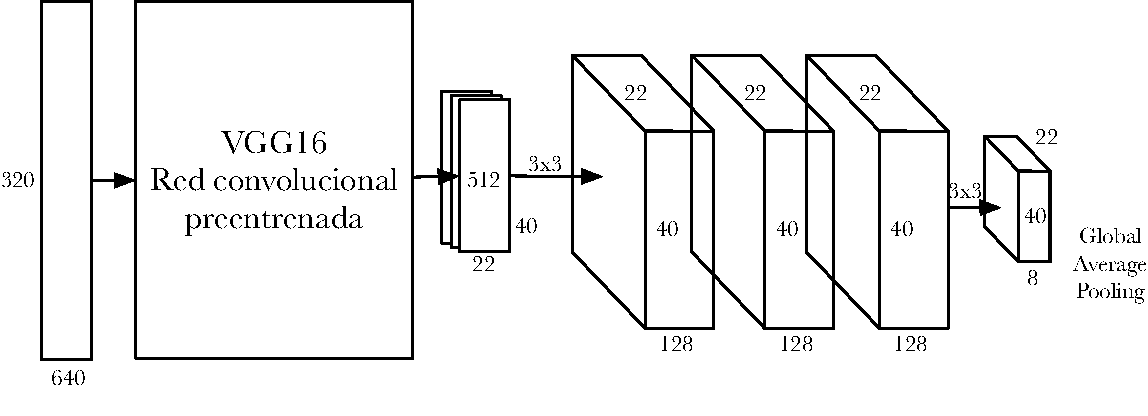
\includegraphics[width=0.7\linewidth]{fcn_arch}}
\end{figure}

De nuevo habrá que transformar el conjunto de datos por medio de la red
convolucional preentrenada, ya que se va a usar un tamaño de imagen de
$360\times640$. Aunque, como se ha comentado, la red convolucional admite un
aumento del tamaño de la imagen sin que crezca exponencialmente el tiempo de
entrenamiento, el entrenamiento de una red convolucional es mucho más costoso
que el de una red clásica. Esto se debe a que hay que actualizar $n\timesn$
pesos por cada píxel de cada imagen. En este caso el entrenamiento de la red
completamente convolucional ha tardado 24 veces más que el entrenamiento de la
red densa del capítulo anterior.

\begin{python}
conv_model.evaluate(test_feat, test_labels)
>>> [0.243715549991, 0.969645081488]
\end{python}

Al evaluar el modelo se ve que consigue una pequeña mejora respecto al modelo
denso. La puntuación en la tabla pública de \textit{Kaggle} para este modelo ha
sido de \textbf{0.8109}.


\subsection{Visualización del modelo}

El trabajar en todo momento (salvo en la última capa) con redes
convolucionales, implica que los pesos son siempre filtros que se aplican a
imágenes. Se pretende entonces conseguir filtros que resalten la existencia en
cada zona de la imagen de un pez de una determinada clase.

Se pueden usar los diferentes valores de los filtros para construir un mapa de
calor para la categoría que le corresponde. Un mapa de calor es una
representación gráfica de los valores de una matriz bidimensional. Generalmente
valores pequeños se asocian a colores más claros, como el azul o el verde, y
valores mayores a colores más cálidos, como el rojo o el morado.

Si se redimensiona el filtro (ya que ha sido reducido por las capas de
\textit{MaxPooling2D}) al tamaño de la imagen original, se puede ver cómo
encuentra el pez a clasificar en cada imagen. Como ejemplo, al aplicar la red a
la imagen de la figura \ref{fc-fish} podemos visualizar el filtro perteneciente
a su categoría (ALB: \textit{Thunnus alalunga}) en la figura \ref{fc-heatmap}.

\begin{figure}
    \caption{Una imagen correspondiente a la clase ALB: \textit{Thunnus alalunga}}
\label{fc-fish}
  \makebox[\textwidth]{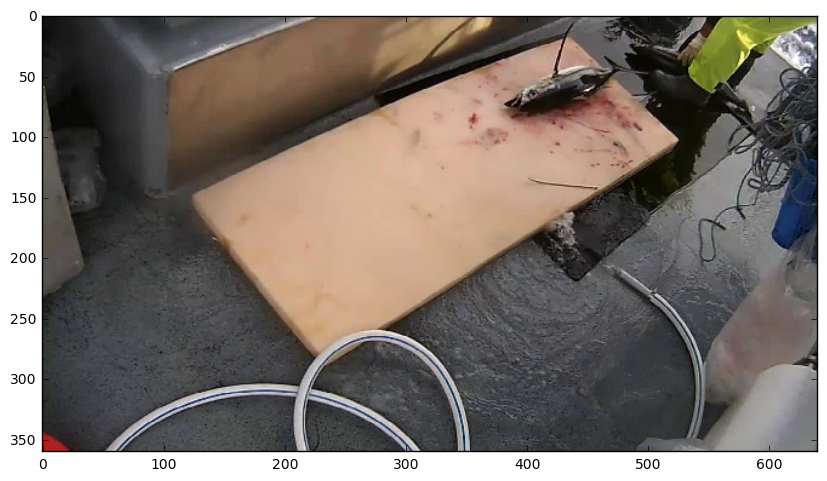
\includegraphics[width=\linewidth]{fc-fish}}
\end{figure}

\begin{figure}
    \caption{Aplicación del mapa de calor reescalado a la imagen de la figura \ref{fc-fish}}
\label{fc-heatmap}
  \makebox[\textwidth]{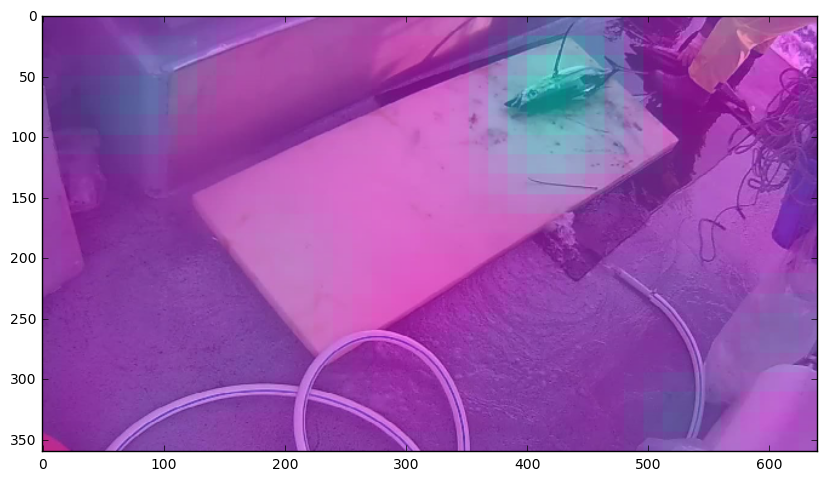
\includegraphics[width=\linewidth]{fc-heatmap}}
\end{figure}

Esto no solo permite comprobar que el modelo funciona correctamente, sino también buscar los ejemplos que peor clasifica y analizar qué está señalando el mapa de calor correspondiente.

Un ejemplo claro de cómo se puede usar esta técnica de visualización para
detectar los errores en el modelo es el intento de clasificación un atún de
cola amarilla (YFT: \textit{Thunnus albacares}), en la imagen de la figura
\ref{yft}. Una característica de los atunes de cola amarilla es su banda de
tonos amarillos en el lomo, característica que el modelo podría haber aprendido
gracias a los ejemplos. Sin embargo, la imagen muestra el atún visto
desde abajo, con las aletas abiertas. Esto esconde una de las principales
características del atún, siendo difícil clasificarlo incluso para un humano no
familiarizado con atunes.

Al mostrar el mapa de calor correspondiente (figura \ref{yft-heatmap}) se puede
apreciar que la hipótesis de que el modelo ha aprendido a detectar los atunes
de cola amarilla a través del color podría ser cierta, ya que una de las partes
más importantes de la foto para el filtro son los pantalones del pescador, de
un color amarillo fuerte.

Esto permite tomar ciertas decisiones sobre el entrenamiento del modelo. Por
ejemplo, si se ve que la fijación del modelo con el color es un error y es
preferible que use otras cosas como formas o texturas, se puede eliminar el
color de las imágenes o aumentar los datos usando transformaciones de color que
hagan especial hincapié en la varianza del color amarillo.

\begin{figure}
    \caption{Una imagen correspondiente a la clase ALB: \textit{Thunnus alalunga}}
\label{yft}
  \makebox[\textwidth]{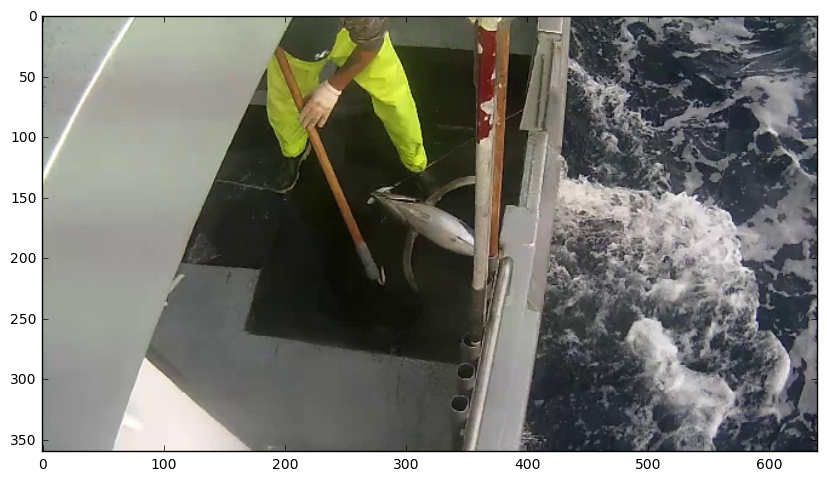
\includegraphics[width=\linewidth]{yft}}
\end{figure}

\begin{figure}
    \caption{Aplicación del mapa de calor reescalado a la imagen \ref{fc-fish}}
\label{yft-heatmap}
  \makebox[\textwidth]{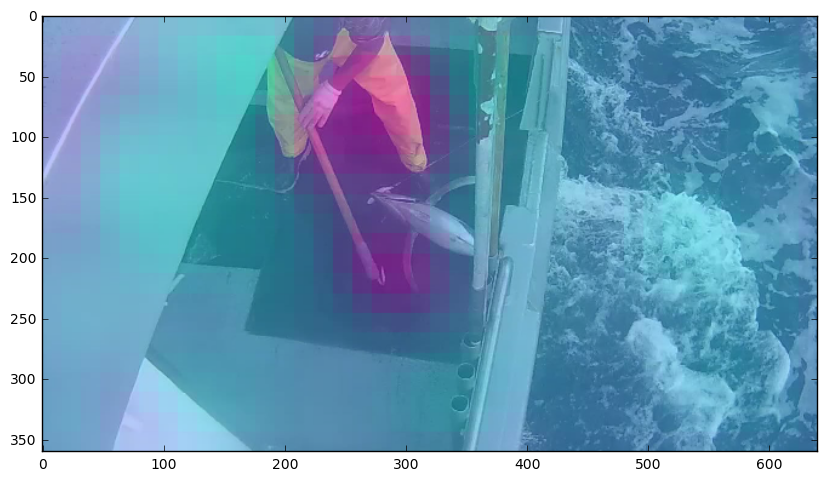
\includegraphics[width=\linewidth]{yft-heatmap}}
\end{figure}

\section{Modelo con entrada múltiple}
\label{sec:multi_entry}

Como se vió en el análisis del conjunto de datos (sección \ref{dataset}), hay
otras propiedades de las imágenes cuyo uso podría permitir una mejora de los
modelos. Por ejemplo, las imágenes están tomadas en diferentes barcos, con
diferentes modelos de cámaras. No todas las cámaras generan imágenes del mismo
tamaño, por lo que se podría averiguar el barco del que se ha tomado la
fotografía por el tamaño de la imagen.

Ya que cada barco suele pescar diferentes tipos de peces con mayor o menor
probabilidad, el conocer el tipo de barco puede ser aprovechado por el modelo
para balancear las posibilidades de cada categoría dependiendo del tipo de
pesca que suela llevar.

La idea no es hacer todo esto a mano, sino entrenar un modelo que tenga en
cuenta tanto las imágenes como otra información válida; en este caso, cual es
el tamaño de la imagen. En el conjunto de datos hay diez tamaños diferentes de
imágenes, las cuales se codificarán en \textit{onehot} para facilitar el
entrenamiento.  Los diferentes tamaños de las imágenes son los indicados en el
cuadro \ref{image_sizes}.

\begin{table}[]
\centering
\caption{Ocurrencia de los diferentes tamaños de imagen}
\label{image_sizes}
\begin{tabular}{rr}
\textbf{Tamaño de la imagen} & \textbf{Cantidad de imágenes} \\
1192 \times 670              & 169                           \\
1276 \times 718              & 192                        \\
1244 \times 700              & 23                            \\
1280 \times 720              & 1880                          \\
1280 \times 750              & 520                           \\
1280 \times 924              & 51                            \\
1280 \times 974              & 344                           \\
1334 \times 750              & 28                            \\
1518 \times 854              & 37                            \\
1732 \times 974              & 33                           
\end{tabular}
\end{table}

Para la arquitectura del modelo vamos a usar la red densa, con la diferencia de
que la última capa tendrá dos entradas: la salida de las capas ocultas de la
red neuronal y la clasificación del tamaño de la imagen, codificado en
\textit{onehot}, como se muestra en la figura \ref{multi_input_arch}.

\begin{figure}
    \caption{Arquitectura del modelo con entrada múltiple}
\label{multi_input_arch}
  \makebox[\textwidth]{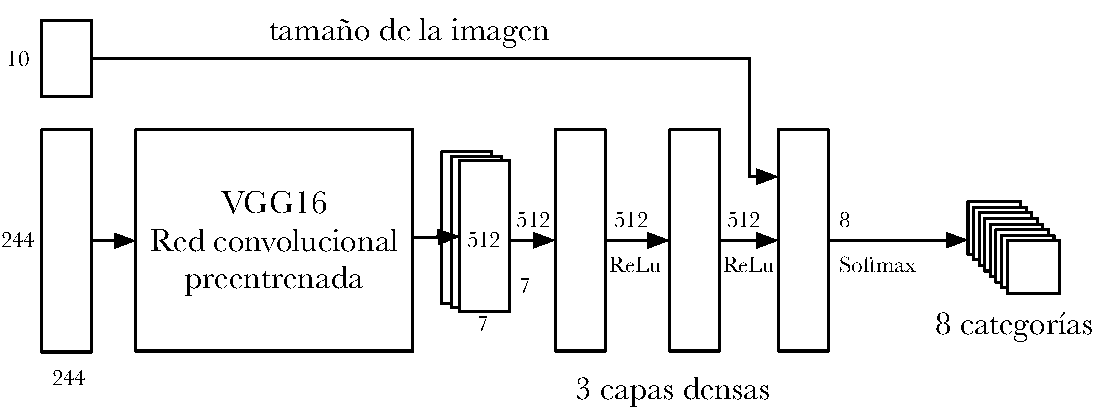
\includegraphics[width=\linewidth]{multi_input_arch}}
\end{figure}

La estructura del código es ligeramente diferente, ya que ahora vamos a generar
todas las capas que teníamos anteriormente menos la última en una misma
función:

\begin{python}
def build_dense_layers(dropout=0.5):
    # Usamos las entradas de la red convolucional, como antes
    inp = Input(conv_layers[-1].output_shape[1:])
    x = MaxPooling2D()(inp)
    x = BatchNormalization(axis=1)
    x = Flatten()
    x = Dropout(dropout/4)
    x = Dense(512, activation='relu')
    x = BatchNormalization()
    x = Dropout(dropout)
    x = Dense(512, activation='relu')
    x = BatchNormalization()
    x = Dropout(dropout/2)
    return x

\end{python}

Usando esta función, añadimos una capa final para la clasificación, cuya entrada
será la union entre la red densa y la información sobre los tamaños de las
imágenes. Esta capa deberá clasificar cada imagen usando tanto la información
disponible de la red densa como el barco al que pertenece.

\begin{python}
# Generar las capas de la red
net = build_dense_layers()

# Usar las entradas de las dimensiones de cada elemento
size_inputs = Input(len(sizes))
bn_inputs = BatchNormalization()(size_inputs)

# Unir las dos entradas en una sola capa
net = merge([net, bn_inputs], 'concat']
net = Dense(8, activation='softmax')(net)

# Crear la red
dense_model = keras.models.Model(
    [inp, size_inputs],  # El modelo ahora tiene multientrada
    net
)
\end{python}

Tras construir el modelo con las entradas múltiples y entrenarlo sobre los dos
conjuntos de entrenamiento (las imágenes y los tamaños de las imágenes) vemos
la evaluación del modelo.

\begin{python}
dense_model.evaluate(test_feat, test_labels)
>>> [0.373333961543, 0.941351055711]
\end{python}

El modelo ha sacado una evaluación peor que modelos anteriores, incluso usando
un modelo que ya se conocía con una evaluación superior.

Aunque la idea es buena, lo que está haciendo por debajo es clasificar los
diferentes barcos en base a los tamaños de sus imágenes. Debido a la amplia
diferencia de las imágenes de los diferentes tipos de barcos, ya sea por los
colores, iluminación, objetos, etc, el anterior modelo denso probablemente ya
esté teniendo en cuenta de qué barco es cada imagen. Por lo tanto lo único que
have el introducir estos datos es añadir complejidad del modelo, haciendo más
difícil que converja a una buena solución.

El envío de este modelo ha obtenido una puntuación de \textbf{1.0466} en la
tabla pública de \textit{Kaggle}, empeorando el anterior envío.

\subsection{Fuga de datos}

En las competiciones de modelos predictivos como \textit{Kaggle} a veces se usan datos no diferentes al conjunto de datos para clasificar. En este caso hemos usado los tamaños de las imágenes, pero podría usarse también información oculta en los metadatos de la imágen, como coordenadas GPS, hora de toma de la fotografía o marca de la cámara. Esto se conoce como \textbf{fuga de datos}.

No todos estos datos son publicados de una manera voluntaria por comunidades de campeonatos, pero son útiles para conseguir una pequeña mejora en el modelo, siempre que el modelo puede aprovecharse de estos datos.

\section{Salida múltiple}

Como vimos anteriormente en la figura \ref{yft-heatmap}, la red completamente
convolucional es capaz de clasificar correctamente la imagen pero por las
razones incorrectas: los pantalones amarillos del pescador. Un modelo que sea
capaz de clasificar la imagen identificando la localización del pez podría
evitar este tipo de errores. Intuitivamente esta idea tiene sentido, ya que es lógico
buscar primero si hay un pez en la imagen y luego distinguir a qué categoría
pertenece.

Al usar técnicas de aprendizaje supervisado como las que estamos usando es
necesario disponer de ejemplos con respuesta conocida para poder entrenar los
modelos. Si queremos un modelo que localice peces en las imágenes necesitaremos
ejemplos con localizaciones conocidas para el conjunto de entrenamiento, cosa
que el conjunto de datos no posee.

Afortunadamente, un usuario ha localizado todos los peces del conjunto de
entrenamiento en rectángulos y ha publicado un conjunto de datos con las
coordenadas de los rectángulos que los contienen. Las reglas de la competición
en \textit{Kaggle} indican que es posible usar conjuntos de datos no oficiales
generados por otras fuentes siempre que estos se hagan públicos y estén
disponibles para todos los participantes.

Usando esta información se va a hacer un modelo que para cada imagen genere una
salida múltiple: la clasificación en una de las ocho categorías y las
coordenadas del rectángulo que contiene al pez.

El conjunto de datos consiste en un archivo \textit{json} con la siguiente estructura.

\begin{python}
{
    "annotations": [
        {
            "class": "rect",
            "height": 79.0,
            "width": 256.0,
            "x": 815.0,
            "y": 124.0
        }
    ],
    "class": "image",
    "filename": "img_07795.jpg"
},
\end{python}

Cada una de las imágenes posee una lista de rectángulos, definidos por su
altura, anchura y las coordenadas del centro. Algunas imágenes poseen varios
peces, por lo que la lista de rectángulos puede contener más de un elemento.

Para ilustrar estos rectángulos y comprobar que están señalando la localización
correctamente se ha pintado un rectángulo con las mismas coordenadas en la
figura \ref{box}. Se puede observar que captura con precisión la localización
del pez.


\begin{figure}
  \caption{Representación de un rectángulo del conjunto de datos auxiliar que ubica cada pez en su imagen}
\label{box}
  \makebox[\textwidth]{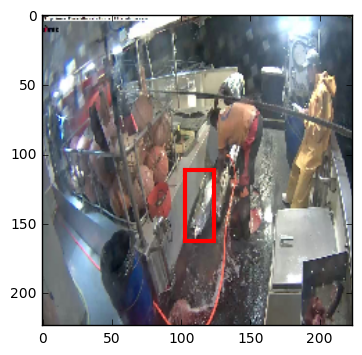
\includegraphics[width=0.5\linewidth]{box}}
\end{figure}


\subsection{Arquitectura del modelo}

Generar la caja que contiene al pez no es un problema de clasificación, porque
no tiene que distinguir entre diferentes tipos de peces, solo tiene que
identificar dónde hay uno. Esto favorecerá que la red busque características
generales de peces, en vez de características generales de cada una de las
categorías. Por otro lado, encontrar la clasificación correcta sí que requiere
buscar características específicas de cada categoría.

Al usar la misma red para ambas tareas, esta deberá encontrar un balance entre
encontrar características específicas de cada categoría y características
generales de los peces.

Para la creación de la red vamos a seguir el mismo procedimiento que en la
entrada múltiple (sección \ref{sec:multi_entry}), solo que en vez de añadir la
entrada extra en la última capa, dividiremos esta última capa en dos redes
diferentes, como se muestra en la figura \ref{multi_output_arch}.

\begin{figure}
  \caption{Arquitectura del modelo denso con salida múltiple}
\label{multi_output_arch}
  \makebox[\textwidth]{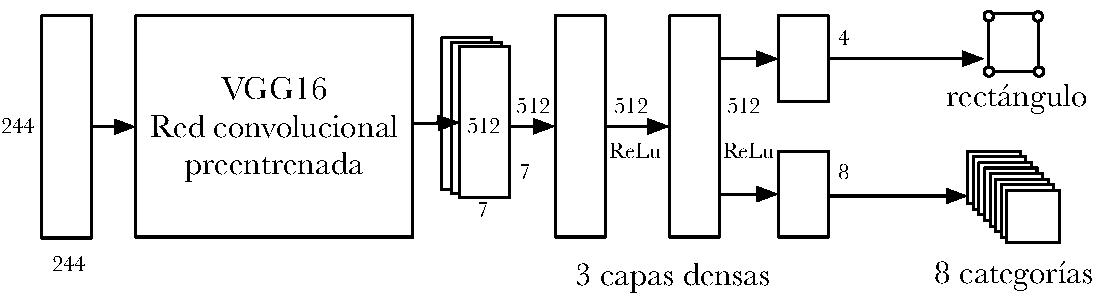
\includegraphics[width=\linewidth]{multi_output_arch}}
\end{figure}


La primera capa de salida, de localización, no posee una función de activación
ya que las cuatro salidas representa las cuatro propiedades con las que
representamos el rectángulo (x, y, altura y anchura) y es necesario que la red
indique el valor de cada una de esas cuatro propiedades.

La segunda capa es la que hemos usado hasta ahora: ocho salidas representando la
codificación \textit{onehot} de las ocho categorías.
\begin{python}
# Generar la red sin la capa de salida 
net = build_dense_layers(dropout)
# Agregar la capa de salida para la localizacion
net_bb = Dense(4, name='bb')(net)
# Agregar la capa de salida para la clasificacion
net_class = Dense(8, activation='softmax', name='class')(net)
# Generar el modelo usando la entrada + ambas capas de salida
model = Model([inp], [net_bb, net_class])
\end{python}

Al entrenar el modelo es necesario indicar de dónde sale el valor a optimizar
en cada una de las salidas. Para la nueva salida vamos a usar el error
cuadrático medio (\textit{MSE}, en inglés) entre los valores del conjunto de
datos de rectángulos y los valores generados. El \textit{MSE} consiste en la
media del cuadrado de la diferencia entre los valores esperados y los valores
de la salida. Esto penalizará mucho más los valores lejanos a la salida
esperada que los pequeños errores.

Ya que el error cuadrático será de una magnitud mayor que la pérdida logarítmica,
se pondera cada una con diferentes pesos.

\begin{python}
model.compile(
    Adam(lr=0.001),
    loss=['mse', 'categorical_crossentropy'],
    metrics=['accuracy'],
    loss_weights=[.001, 1.],  # Ponderar los errores
)
\end{python}

Ahora hay que proporcionar los ejemplos de las salidas de cada uno de los
conjuntos de datos para cada capa de salida, así como para el conjunto de
validación.

\begin{python}
model.fit(
    conv_feat,
    [trn_bbox, trn_labels],
    batch_size=batch_size,
    nb_epoch=7,
    validation_data=(conv_val_feat, [val_bbox, val_labels]),
)
\end{python}

La evaluación del modelo sobre el conjunto de test generará una evaluación para
cada capa de salida. En el cuadro \ref{eval_multi} podemos ver los valores de
cada una de las capas de salida.

\begin{table}[]
\centering
\caption{Resultados de la evaluación del modelo de salida múltiple sobre el
conjunto de test}
\label{eval_multi}
\begin{tabular}{rrr}
                       & \textbf{Pérdida} & \textbf{Precisión} \\
\textbf{Localización}  & 239.54                        & 0.8454             \\
\textbf{Clasificación} & 0.2403                        & 0.9698            
\end{tabular}
\end{table}

La precisión de la capa de clasificación, que es la que vamos a usar para la
competición, es la más alta hasta ahora. Esto puede deberse a que, como
decíamos al principio de esta sección, tiene que conseguir características para
distinguir peces así como caracterísiticas de cada categoría.

La puntuación en la tabla pública de \textit{Kaggle} para este modelo ha sido
de \textbf{0.8675}, siendo el segundo mejor modelo de los entrenados hasta ahora.

\subsection{Visualización de la localización de peces}

Como se veía en la imagen \ref{box} se puede representar la localización anotada
en el conjunto de datos de cada imagen. De la misma manera, podemos visualizar
los valores de salida de la capa de localización para ver si el modelo es capaz
de encontrar dónde se encuentra cada pez en la imagen.

En la figura \ref{predicted_boxes_1} podemos ver en rojo la localización original
y en verde la generada por el modelo. Aunque no es perfecta, captura
aproximadamente dónde se encuentra el pez. Es curioso notar que en la primera de
las dos imágenes solo está encontrando las características más visibles del pez.
La cola, que casi no es distinguible, no se incluye dentro del rectángulo
generado por el modelo.

En la segunda imagen el modelo ha sido capaz de identificar un pez, pero no el que
se le había indicado en el conjunto de entrenamiento. El pez que ha localizado
es más visible y está mejor iluminado, por lo que es más fácil de localizar. El pez
original está parcialmente tapado por la cabeza de un pescador.

\begin{figure}
  \caption{En rojo, el rectángulo correspondiente a la localización del pez en
  el conjunto de datos alternativo. En verde, el rectángulo generado por el
  modelo con salida múltiple.}
\label{predicted_boxes_1}
  \makebox[\textwidth]{
  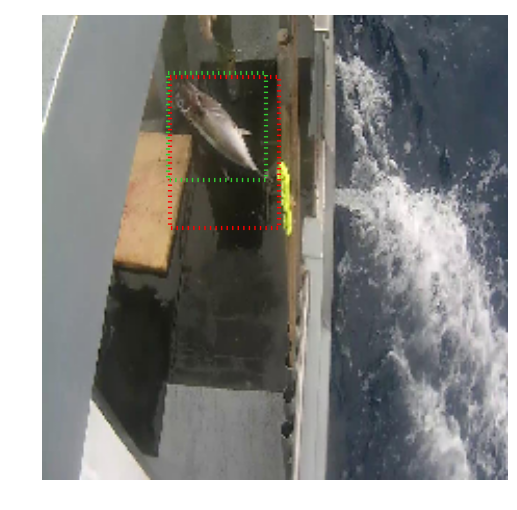
\includegraphics[width=0.5\linewidth]{predicted_boxes_1}
  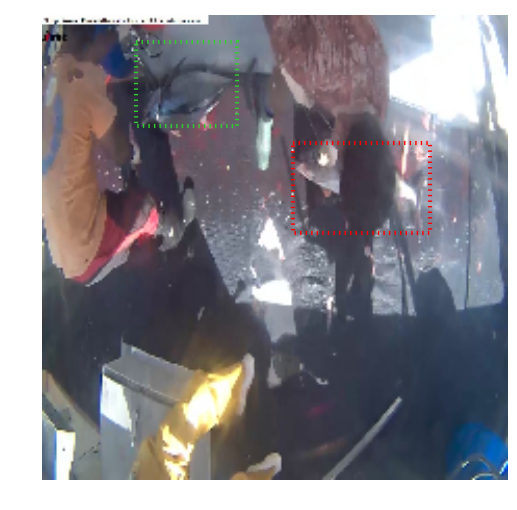
\includegraphics[width=0.5\linewidth]{predicted_boxes_2}
  }
\end{figure}


\section{Modelos \textit{ensemble}}

En competiciones de modelos predictivos es habitual que la mejor puntuación
no la obtenga un único modelo, sino un modelo construido combinando varios. Este
tipo de modelos se conocen como \textit{ensemble models} (modelos de conjunto).

Para generar estos modelos no es necesario reentrenar los modelos disponibles,
sino trabajar con las salidas de estos. Primero calculamos las predicciones de
cada modelo que queremos combinar. Luego generamos una predicción del modelo
\textit{ensemble} agregando los valores de las predicciones. Hay otros métodos
para construir modelos \textit{ensemble} más sofisticados, pero aquí se van a
considerar únicamente los más simples:

\begin{itemize}
    \item{\textbf{Votación:} La salida de cada modelo se entiende como una
            votación de a qué categoría debería pertenecer dicha entrada. La
            salida del modelo final es la elección ganadora de esa votación. Por
            ejemplo, si el modelo 1 ha elegido ALB y los modelos 2 y 3 han
        elegido YFT, la salida del modelo \textit{ensemble} será YFT.}
    \item{\textbf{Media ponderada:} En el caso de que la salida sean
            probabilidades de cada clase se puede  usar una media ponderada
            entre los valores de los modelos. La ponderación de la media permite
            dar preferencia al modelo con más confianza.
            
            En el cuadro \ref{ensemble_sample} podemos ver un ejemplo de cómo
        sería la salida de un modelo \textit{ensemble} ejemplo usando una media
    aritmética entre tres modelos diferentes.}

Debido a que los modelos presentados generan un vector de probabilidades para
cada categoría, los modelos \textit{ensemble} generados usarán la media
ponderada.

\begin{table}[]
\centering
\caption{Predicciones de diferentes modelos para una imagen, unidas en un modelo
final mediante una media aritmética}
\label{ensemble_sample}
\begin{tabular}{rllllllll}
Modelo              & ALB   & BET   & DOL   & LAG   & NoF   & OTHER & SHARK  & YFT  \\
\hline
Salida múltiple     & 0.010 & 0.052 & 0.030 & 0.001 & 0.123 & 0.079 & 0.046 & 0.875\\
Red base            & 0.020 & 0.001 & 0.030 & 0.002 & 0.123 & 0.079 & 0.046 & 0.844\\
Red convolucional   & 0.030 & 0.301 & 0.029 & 0.001 & 0.123 & 0.079 & 0.046 & 0.502\\
\hline
Ensemble            & 0.020 & 0.118 & 0.030 & 0.001 & 0.123 & 0.079 & 0.046 & 0.740
\end{tabular}
\end{table}

Usar la pérdida logarítmica como métrica hace que se castigue mucho las bajas
probabilidades en las categorías correctas. Usar la media para estos modelos
puede ayudar a evitar este comportamiento, ya que solo tendrán probabilidades
cercanas a cero aquellas categorías que sean casi cero en todos los modelos.

Un ejemplo puede verse en la categoría LAG del cuadro \ref{ensemble_sample}.
Todas los modelos predicen una baja puntuación para esa categoría, por lo que la
puntuación final también es muy baja. Sin embargo en la categoría BET existe un
modelo que le da una puntuación media, haciendo que esta se aleje de cero. En
cuanto uno de los modelos no está de acuerdo en que la puntuación sea cero, esta
se aleja.

\subsection{Resultados}

Se han presentado dos modelos diferentes usando esta técnica. Ambos modelos
están compuestos de tres modelos anteriores:

\begin{itemize}
    \item{Modelo con clasificador denso, dropout, normalización por lotes y
        aumento de datos.}
    \item{Modelo completo convolucional}
    \item{Modelo con salida múltiple}
\end{itemize}

Estos tres modelos son los que mejores resultados obtuvieron previamente, así
que se usarán para generar dos modelos. El primero usará la media aritmética de
la salida mientras que el segundo será ponderado de la siguiente manera: 25 \%
para el clasificador denso, 25 \% para el modelo con salida múltiple y 50 \%
para el modelo completo convolucional.

Al evaluar estos modelos en \textit{Kaggle}, los resultados de la tabla pública
son los siguientes

\begin{itemize}
    \item{Media aritmética sobre los tres modelos: \textbf{0.9175}
    \item{Media ponderada favoreciendo el modelo completo convolucional: \textbf{0.8975}
\end{itemize}

Desafortunadamente las puntuaciones de \textit{ensemble}, que tradicionalmente suelen conseguir las mejores posiciones en las competiciones de \textit{Kaggle}, no han conseguido ser las mejores.

\section{Modelos finales presentados}

En los cuadros \ref{model_id} y \ref{final_scores} se presenta un resumen de
los modelos presentados, junto a sus puntuaciones.

Las reglas de la competición establecen que solo es posible puntuar dos modelos
en la tabla de puntuaciones privada y solo es posible usar un modelo para la
segunda fase.

El mejor modelo según las puntuaciones públicas de la primera fase es el que
usa un clasificador convolucional en las últimas capas, seguido del que usa una
salida múltiple para intentar clasificar los peces. Hay que recordar que estas
puntuaciones se calculan usando un subconjunto del conjunto de test, por lo que
puede cambiar cuando se publique la tabla privada.

Tradicionalmente los modelos \textit{ensemble} consiguen mejores puntuaciones
en las competiciones de \textit{Kaggle}, por lo que se ha decidido enviar un
modelo \textit{ensemble} (el tercero en mejor puntuación) y el convolucional
completo.

Al publicarse las puntuaciones privadas, vemos en el cuadro \ref{final_scores}
que el modelo convolucional consigue mejor puntuación, así que es seleccionado
como el modelo final a enviar.

La puntuación final de este modelo es de \textbf{0.907} en la tabla pública y
\textbf{1.998} en la privada, consiguiendo una posición 210 de 2293
participantes y una medalla de bronce (por clasificar dentro del mejor 10 \% de
los participantes).

\begin{table}[]
\centering
\caption{Identificadores de los modelos}
\label{model_id}
\begin{tabular}{rl}
\textbf{Id} & \textbf{Modelo}                                                       \\ \hline
vgg         & VGG16 con ajuste fino                                                 \\
v-512       & VGG16 con capas de 512 salidas                                        \\
v-norm      & VGG16 con normalización por lotes (+ 512 s, \textit{dropout})       \\
v-aug       & VGG16 con aumento de datos (+ 512 s, \textit{dropout}, norm.)       \\
v-fcn       & VGG16 con red convolucional (+ norm.)                                 \\
m-in        & VGG16 con entrada múltiple (+ 512 s, \textit{dropout}, norm, datos) \\
m-out       & VGG16 con salida múltiple (+ 512 s, \textit{dropout}, norm, datos)  \\
e-arit      & \textit{Ensemble} con media aritmética                              \\
e-pond      & \textit{Ensemble} con media aritmética ponderada                   
\end{tabular}
\end{table}

\begin{table}[]
\centering
\caption{Identificadores de los modelos}
\label{final_scores}
\begin{tabular}{r|lllll}
\textbf{Id}           & \textbf{Local}        & 1ª fase                      &                              & 2ª fase                      &                              \\ \cline{3-6} 
\multicolumn{1}{l|}{} & \multicolumn{1}{l|}{} & \multicolumn{1}{l|}{Pública} & \multicolumn{1}{l|}{Privada} & \multicolumn{1}{l|}{Pública} & \multicolumn{1}{l|}{Privada} \\ \hline
vgg                   & 2.383                 & 2.632                        & -                            & -                            & -                            \\
v-512                 & 1.272                 & 2.381                        & -                            & -                            & -                            \\
v-norm                & 0.451                 & 1.017                        & -                            & -                            & -                            \\
da-aug                & 0.312                 & 0.936                        & -                            & -                            & -                            \\
fcn                   & 0.243                 & 0.811                        & 0.770                        & 0.907                        & 1.998                        \\
m-in                  & 0.373                 & 1.047                        & -                            & -                            & -                            \\
m-out                 & 0.240                 & 0.867                        & -                            & -                            & -                            \\
e-arit                & -                     & 0.917                        & -                            & -                            & -                            \\
e-pond                & -                     & 0.897                        & 0.841                        & -                            & -                           
\end{tabular}
\end{table}
 
% Chapter 1

\chapter{Conclusiones} % Main chapter title
\label{chap:conclusiones} % For referencing the chapter elsewhere, use \ref{Chapter1} 

El objetivo principal de este trabajo era afrontar un problema real en una de
las competiciones \textit{\textbf{featured}} de \textit{Kaggle}, incluso
aspirar a conseguir un premio.

Ha sido un trabajo muy interesante, ya que he aprendido las dificultades
de la implementación de redes de aprendizaje profundo en problemas del
mundo real. Esto requiere enfrentarse a problemas que no aparecen en la teoría.

Las tres principales dificultades encontradas han sido las siguientes:

\begin{itemize}
    \item{\textbf{Cómo afrontar el problema:}
     Hasta el momento había leído bastante sobre
    técnicas de reconocimiento visual usando herramientas fijas que permitían poca
    soltura y por supuesto sin usar ningún tipo de aprendizaje automático.

    Esto se solucionó gracias a la gran comunidad de participantes de
    \textit{Kaggle}. Es de esperar que en una competición con buenos premios
    existan reticencias a ayudar al resto de participantes, pero resultó ser al
    revés. Hay una comunicación permanente en los foros de la competición de las
    técnicas que se están usando, referencias, lecturas, etc. Quiero destacar aquí
    las aportaciones de Felix Yu \parencite{felixyu} y de Jeremy Howard
    \parencite{fastai}. Incluso publicando después de haber terminado la
    competición he entendido otros pasos a seguir que estaba perdiendo. }

    \item{\textbf{Trabajar con grandes cantidades de datos:}
    Los 13000 ejemplos de la segunda fase de la competición hicieron que muchos de
    mis modelos no funcionasen, ya que la máquina se quedaba sin suficiente memoria
    RAM. Esto me hizo tener que \textbf{cuidar la gestión de memoria}, saber
    descargar datos cuando no se están usando y guardar cálculos en disco para no
    tener que repetirlos.  }

    \item{\textbf{Automatización de procesos:}
    La segunda fase de la competición tenía un conjunto de datos de prueba
    desconocido que iba a tener que ser clasificado por un modelo fijo. Esto
    hizo tener que automatizar toda la parte del tratamiento de datos para el
    problema.  }

\end{itemize}

La conclusión principal que saco de este trabajo es la potencia de las redes
convolucionales. Han mejorado cualquier expectativa que tenía sobre el reconocimento
de imágenes y es posible que vayan a convertirse en la base de la visión artificial
en el futuro.

Creo que se pueden abordar muchos problemas diferentes de clasificación de
imágenes usando una arquitectura común que use las modificaciones
realizadas en este problema (\textit{dropout}, normalización por lotes, aumento
de datos, etc).

\section{Kaggle}

Participar en esta competición de Kaggle ha sido divertido y didáctico ya que,
aunque hubiera una competición por un premio, los participantes siempre han
estado dispuestos a ayudarse entre ellos. Creo que dedicarle tiempo a una
competición tiene sus recompensas, independientemente si se gana o no el premio.

Por otro lado, he notado que a la organización promotora (\textit{The Nature
Conservancy}) le falta un poco de experiencia en \textit{Kaggle}. Esto se ha
notado en diferentes detalles. La comunicación en el foro de la plataforma no
ha sido del todo fluida, lo cual ha provocado algunos errores que no tenían que
haberse cometido, como por ejemplo descalificación del mejor clasificado.

Otro ejemplo es la falta de diversidad del conjunto de datos de entrenamiento.
Era muy difícil extraer información de determinados peces con muy poca información,
haciendo complicado hacer modelos que generalizaran correctamente.

Un ejemplo de esto es que el archivo de ejemplo de envío (sección
\ref{submission-sample}), que contiene en cada elemento la misma predicción (la
proporción de ejemplos de cada categoría, normalizado) haya conseguido medalla
de plata, acabando en la posición 33.

\subsection{Puntuación final}

Aunque se le haya dado varias vueltas a usar las capas densas como
clasificadores finales del modelo, el ganador ha sido el que no las usa: el
modelo completamente convolucional. Creo que esto puede ser debido a que es
capaz de, en esas últimas capas convolucionales, detectar elementos más
generales de la imagen, descartando así el ruido que pueden producir los fondos
de la imagen.

\section{Siguientes pasos}

Las siguientes mejoras de este problema creo que vienen reduciendo el ruido generado por todos los elementos de las imágenes que no son peces. Para esto habría primero que recortar automáticamente los peces de las imágenes y entrenar un nuevo modelo con dichas imágenes, pero para esto habría que tener un buen modelo de localización, ya que errar en la localización hará que se clasfiquen ejemplos incorrectamente.

Por otro lado creo que también existe una posible mejora usando diferentes conjuntos de datos, como imágenes de peces sacadas de otras fuentes. De esta manera el modelo sería capaz de aprender características de los peces que no aparecen en los ejemplos.

%\include{Chapters/Chapter3}
%\include{Chapters/Chapter4} 
%\include{Chapters/Chapter5} 

%----------------------------------------------------------------------------------------
%	THESIS CONTENT - APPENDICES
%----------------------------------------------------------------------------------------

\appendix % Cue to tell LaTeX that the following "chapters" are Appendices

% Include the appendices of the thesis as separate files from the Appendices folder
% Uncomment the lines as you write the Appendices

% Appendix A

\chapter{Infraestructura} 
\label{ap:hardware}

\section{Requisitos}

Al principio de este trabajo se comentó que era necesario un enfoque de desarrollo rápido para probar diferentes ideas y encontrar rápidamente los errores y mejoras. Los algoritmos de aprendizaje sobre redes convolucinoales son tradicionalmente costosos en cómputo, por lo que es una dificultad a superar si queremos una evolución rápida de la solución.

\section{Hardware}

\textit{Keras} permite aumentar la velocidad de entrenamiento usando el
procesador gráfico del sistema, siempre que este sea compatible con CUDA \parencite{cuda}.
Para este problema se han usado dos equipos diferentes, ambos compatibles con
CUDA.

Para la mayoría de entrenamientos y experimentos se ha usado un ordenador con las siguientes características:

\begin{itemize}
    \item{Procesador: Intel i3, 2.7 GHz}
    \item{Procesador gráfico: Nvidia GeForce GTX 950, 2GB de memoria}
    \item{16 GB de RAM}
\end{itemize}

Este equipo era suficiente para la mayoría de entrenamientos. Sin embargo cuando era necesario entrenar un conjunto de datos más grande, como la segunda fase de la clasificación, con 13000 ejemplos, el equipo tardaba demasiado en entrenar algunos modelos.

Por eso se optó por buscar una solución en la nube que permitiese alquilar una potencia gráfica superior durante tiempo limitado. Al final se ha optado por las máquinas virtuales de \textit{Amazon AWS}, que permite contratar máquinas por horas. Una de ellas, identificada \textit{p2.xlarge}, ofrece las siguientes características:

\begin{itemize}
    \item{Procesador: Intel i7, 3.5 GHz, 4 núcleos}
    \item{Procesador gráfico: Nvidia Tesla K80}
    \item{61 GB de RAM}
\end{itemize}

Este equipo, con un precio de 0.80 euros la hora, ofrece potencia más que suficiente para entrenar grandes cantidades de datos rápidamente.


%% Appendix A

\chapter{\textit{Keras}} 
\label{ap:keras}

\textit{Keras} es una API escrita en \textit{Python} para el desarrollo de
redes neuronales capaz de ejecutarse en sistemas como \textit{TensorFlow} o
\textit{Theano}. Fue desarrollada con la idea de permitir una experimentación
sencilla y un desarrollo rápido con redes neuronales. Posee soporte para redes
neuronales recurrentes y convolucionales, así como combinaciones de ambas.
También es capaz de aprovechar la GPU para acelerar el entrenamiento de las
redes.


\section{Instalación} 

Para la instalación de \textit{Keras} primero es necesario instalar uno de los
diferentes \textit{frameworks} con los que \textit{Keras} trabaja: \textit{Theano} o
\textit{TensorFlow}. En este caso se ha trabajado con \textit{Theano}, ya que
es un sistema más antiguo y que dispone de más documentación. Para la
instalación se usará \textit{Conda}, un gestor de paquetes para
\textit{Python}. Otros métodos de instalación y posibles soluciones a problemas
se pueden encontrar en la documentación de \textit{Theano} \parencite{theano}.

\begin{python}
>>> conda install theano pygpu
\end{python}

Una vez instalado \textit{Theano} es necesario instalar \textit{Keras}, también
usando \textit{Conda}.

\begin{python}
>>> conda install keras
\end{python}


\section{Uso} 

El uso de la herramienta se puede divivir en tres partes: generación de la red
neuronal, carga del conjunto de datos y entrenamiento y evaluación del modelo.
Aquí se explicarán las partes más usadas en este trabajo, pero es posible
obtener una descripción más precisa en la documentación de \textit{Keras}
\parencite{keras_doc}.

\subsection{Arquitectura}

Lo más importante del uso de \textit{Keras} es ser capaz de definir la
arquitectura de la red. Para ello existe la clase \texttt{Sequential}. Esta
clase representa un conjunto lineal de capas dentro de la red. Como ya hicimos
en la sección \ref{sec:model_connected}, vamos a crear un objeto
\texttt{Sequential} pasando las capas de las que se compondrá la red mediante
objetos.

\begin{python}
from keras.models import Sequential
red_neuronal = Sequential([
    Dense(512, activation='relu'),
    Dense(512, activation='relu'),
    Dense(8, activation='softmax')
    ])
\end{python}

Existen muchos tipos de objetos capa, cada uno representando una variación de
un concepto diferente en la red neuronal. Algunos de los usados en este trabajo
son los siguientes:

\begin{itemize}
    \item{\texttt{Dense}: Capa densa, complemtamente conectada. Las capas usadas en las redes neuronales clásicas.}
    \item{\texttt{Convolution2D}: Capa convolucional. Existen con 1, 2 ó 3 dimensiones.
    \item{\texttt{Dropout}: Aplicación de dropout (sección \ref{sec:dropout}) a la salida de la capa anterior.}
    \item{\texttt{MaxPooling2D}: Capa de muestreo. Elige la mayor de cada cuatro entradas que entren.
    \item{\texttt{BatchNormalization}: Capa de normalización por lotes.
\end{itemize}

Cada capa incluye el tamaño de salida de la capa y una función de activación,
que debe indicarse en el parámetro \texttt{activation}.

Por último, para terminar de crear la red, hay que configurar el aprendizaje de
esta. Esto se hace usando la utilidad \texttt{compile}, que necesita tres
parámetros:

\begin{itemize}
    \item{Optimizador: Mecanismo de optimización, como por ejemplo SGD (descenso de gradiente estocástico).}
    \item{Función de pérdida: Este es el objetivo que el modelo tratará de minimizar. En nuestro caso será \textit{\texttt{'logloss'}}, la pérdida logarítmica.}
    \item{Métricas: Las diferentes métricas que queremos que muestre en la evaluación, además de la función de pérdida}
\end{itemize}


\begin{python}
red_neuronal.compile(
    optimizer='rmsprop',
    loss='categorical_crossentropy',
    metrics=['accuracy'],
)
\end{python}

\subsection{Carga de datos}

Para este proyecto hemos tenido que cargar grandes cantidades de imágenes.
Keras necesita los datos de entrenamiento como matrices de la biblioteca
numérica \textit{numpy}, sin embargo las imágenes están en formato
\textit{jpg}.

La utilidad para convertir imágenes a matrices se llama
\texttt{ImageDataGenerator}. Lo interesante de esta utilidad es que no solo
permite leer archivos y convertirlos, sino que lo hace como un generador. Un
generador en \textit{Python} va devolviendo más elementos a medida que estos son
consumidos. Esto evita tener que generar todos las matrices al mismo tiempo y
cargarlas en memoria. También permite aplicar otras transformaciones a la
imagen para crear un aumento de datos.

\begin{python}
from keras.preprocessing.image import ImageDataGenerator
base_generator = ImageDataGenerator(featurewise_center=False,
    samplewise_center=False,
    featurewise_std_normalization=False,
    samplewise_std_normalization=False,
    zca_whitening=False,
    zca_epsilon=1e-6,
)
\end{python}

Una vez configurada la herramienta hay que llamarla en el directorio sobre el que se quiere actuar.

\begin{python}
image_generator = base_generator.flow_from_directory(
    'data/train',
    target_size=(150, 150),
    batch_size=32,
)
\end{python}

\subsection{Entrenamiento y evaluación}

El entrenamiento del modelo se realiza con la función \texttt{fit}. Es
necesario proveer a la función de los ejemplos de entrada con sus salidas
esperadas (\texttt{data} y \texttt{labels} en nuestro ejemplo). Se le indica
también el número de iteraciones a realizar.

\begin{python}
data, labels = image_generator.flow_from_directory(...)
red_neuronal.fit(data, labels, epochs=10, batch_size=32)
\end{python}

Esto actualizará los pesos de la red para minimizar la función de pérdida
indicada. Una vez finalizado podemos hacer una evaluación del modelo usando
otro conjunto de datos (generalmente el de test) con la función
\texttt{evaluate}. Esta función devolverá la pérdida del modelo sobre el
conjunto más el resto de métricas que se hayan definido.

\begin{python}
red_neuronal.evaluate(test_data, test_labels)
>>> [1.90571456890184755 , 0.66099843993759748]
\end{python}

Para una mayor compresión de como usar esta librería es mejor dirigirse a la documentación \parencite{keras_doc}.


%\include{Appendices/AppendixC}

%----------------------------------------------------------------------------------------
%	BIBLIOGRAPHY
%----------------------------------------------------------------------------------------

\printbibliography[heading=bibintoc]

%----------------------------------------------------------------------------------------

\end{document}  
